%%%%%%%%%%%%%%%%%%%%%%%%%%%%%%%%%%%%%%%%%
% Short Sectioned Assignment LaTeX Template Version 1.0 (5/5/12)
% This template has been downloaded from: http://www.LaTeXTemplates.com
% Original author:  Frits Wenneker (http://www.howtotex.com)
% License: CC BY-NC-SA 3.0 (http://creativecommons.org/licenses/by-nc-sa/3.0/)
%%%%%%%%%%%%%%%%%%%%%%%%%%%%%%%%%%%%%%%%%

%----------------------------------------------------------------------------------------
%	PACKAGES AND OTHER DOCUMENT CONFIGURATIONS
%----------------------------------------------------------------------------------------

\documentclass[paper=a4, fontsize=11pt]{scrartcl} % A4 paper and 11pt font size

% ---- Entrada y salida de texto -----

\usepackage[T1]{fontenc} % Use 8-bit encoding that has 256 glyphs
\usepackage[utf8]{inputenc}
%\usepackage{fourier} % Use the Adobe Utopia font for the document - comment this line to return to the LaTeX default

% ---- Idioma --------

\usepackage[spanish, es-tabla]{babel} % Selecciona el español para palabras introducidas automáticamente, p.ej. "septiembre" en la fecha y especifica que se use la palabra Tabla en vez de Cuadro

% ---- Otros paquetes ----

\usepackage{url} % ,href} %para incluir URLs e hipervínculos dentro del texto (aunque hay que instalar href)
\usepackage{amsmath,amsfonts,amsthm} % Math packages
%\usepackage{graphics,graphicx, floatrow} %para incluir imágenes y notas en las imágenes
\usepackage{graphics,graphicx, float, subfig} %para incluir imágenes y colocarlas

% Para hacer tablas comlejas
%\usepackage{multirow}
%\usepackage{threeparttable}

%\usepackage{sectsty} % Allows customizing section commands
%\allsectionsfont{\centering \normalfont\scshape} % Make all sections centered, the default font and small caps

\usepackage{fancyhdr} % Custom headers and footers
\pagestyle{fancyplain} % Makes all pages in the document conform to the custom headers and footers
\usepackage{eurosym} % Para poder añadir el símbolo del euro
\fancyhead{} % No page header - if you want one, create it in the same way as the footers below
\fancyfoot[L]{} % Empty left footer
\fancyfoot[C]{} % Empty center footer
\fancyfoot[R]{\thepage} % Page numbering for right footer
\renewcommand{\headrulewidth}{0pt} % Remove header underlines
\renewcommand{\footrulewidth}{0pt} % Remove footer underlines
\setlength{\headheight}{13.6pt} % Customize the height of the header

\numberwithin{equation}{section} % Number equations within sections (i.e. 1.1, 1.2, 2.1, 2.2 instead of 1, 2, 3, 4)
\numberwithin{figure}{section} % Number figures within sections (i.e. 1.1, 1.2, 2.1, 2.2 instead of 1, 2, 3, 4)
\numberwithin{table}{section} % Number tables within sections (i.e. 1.1, 1.2, 2.1, 2.2 instead of 1, 2, 3, 4)

\setlength\parindent{0pt} % Removes all indentation from paragraphs - comment this line for an assignment with lots of text

\newcommand{\horrule}[1]{\rule{\linewidth}{#1}} % Create horizontal rule command with 1 argument of height
  % Configuración del documento

%----------------------------------------------------------------------------------------
%	TÍTULO Y DATOS DE LOS ALUMNOS
%----------------------------------------------------------------------------------------

\title{	
	\normalfont \normalsize 
	\textsc{\textbf{Inteligencia de Negocio (2019-2020)} \\ Doble grado en Informática y Matemáticas \\ Universidad de Granada} \\ [25pt] 
	\horrule{0.5pt} \\[0.4cm]
	\huge Práctica 2: Análisis Relacional mediante Segmentación \\ 
	\horrule{2pt} \\[0.5cm] 
}

\author{Alberto Jesús Durán López \\
		DNI: 54142189-M \\
		Email: albduranlopez@correo.ugr.es \\
		Grupo Prácticas: Lunes} 
\date{\normalsize\today}

%----------------------------------------------------------------------------------------
% DOCUMENTO
%----------------------------------------------------------------------------------------
\lstset{
	basicstyle=\fontsize{10}{10}\selectfont\ttfamily
}

\begin{document}
	\maketitle       % título
	\newpage 
	\tableofcontents % índice
	\newpage
	
	
	
	
	\section{Introducción}
	
	En esta práctica veremos el uso de técnicas de aprendizaje no supervisado para análisis relacional mediante segmentación. Se trabajará con un conjunto de datos sobre el que se aplicarán distintos algoritmos de agrupamiento (clustering).
	
	Trabajaremos con el archivo \texttt{mujeres\_fecundidad\_INE\_2018.csv}, un estudio publicado por el instituto Nacional de Estadística (INE), el cual recoge información de diferentes campos para el estudio de la fecundidad de las mujeres.
	
	El documento dispone de un conjunto de 14.556 respuestas con un total de 463 variables sobre datos de la vida de cada mujer.
	Segmentaremos la población seleccionando previamente grupos de interés. (estado civil, trabajo, nº hijos...etc) donde estudiaremos 3 casos aplicándole los algoritmos de clustering. 
	
	A partir de los resultados extraeremos las conclusiones sobre los grupos de población. \\
	
	
	Toda la información referente a esta práctica se puede encontrar en la página web de la asignatura: \href{url}{http://sci2s.ugr.es/graduateCourses/in} \\
	
	Comenzaremos explicando brevemente los algoritmos de clustering usados.
	
	\begin{itemize}
		\item \texttt{AgglomerativeClustering}: Realiza una agrupación jerárquica utilizando un enfoque ascendente: cada observación comienta en su propio cluster y sucesivamente, los clusters se van fusionando juntos. El criterio de vinculación determina la métrica usada para la estrategia de fusión. Al ser jerárquico mostraremos su dendograma.
		\item \texttt{Meanshift}: Tiene como objetivo descubrir \textit{manchas} en una densidad uniforme de muestras. Es un algoritmo basado en centroides que funciona actualizando los candidatos a centroides para ser la media de los puntos dentro de una determinada región. Luego, estos cansidatos se filtran en una etapa post-procesamiento para eliminar los duplicados y así formar el conjunto final de centroides.
		\item \texttt{KMeans}: Agrupa los datos tratando se deparar muestras en n grupos de igual varianza, minimizando el criterio conocido como inercia o suma de cuadrados. Este algoritmo requiere que se especifique el número de clusters. Escala bien en muestras grandes y en la historia ha sido usado en numerosas áreas y aplicaciones de diferentes campos.
		\item \texttt{DBSCAN}: Este algoritmo considera los clústers como áreas de alta densidad separadas por áreas de baja densidad. Debido a este hecho, los clusters en DBSCAN pueden tener cualquier forma, a diferencia de Kmeans que asume que los clusters tienen forma convexa. El componente central de este algoritmo es el concepto de muestras de núcleo, que son muestras que están en áreas de alta densidad.
		\item \texttt{MiniBatchKMeans}:Es una variante del algoritmo KMeans que utiliza \textit{mini lotes/batches} para reducir el tiempo de ejecución mientras intenta optimizar la misma función objetivo. Los \textit{mini lotes} son subconjuntos de los datos de entrada muestreamos aleatoriamente en cada iteración de entrenamiento. Estos \textit{mini lotes} reducen drásticamente la cantidad de cómputo requerida para converger a una solución local. 
	\end{itemize}


	Mostraremos un dendograma para el algoritmo \texttt{AgglomerativeClustering}, así como un heatmap, kplot, boxplot y scatter matriz para las combinaciones \{Caso de estudio-Algoritmo\}	
	
	
	
	Por otro lado, calcularemos las métricas \textit{Calinski Harabasz} y \textit{Silhouette}, llamadas en la función \texttt{CalcularMetricas}:
	
	\begin{itemize}
		\item \texttt{Calinski Harabasz}: Conocido como \textit{Variance Ratio Criterion} o \textit{Criterio de relación de varianza}. 
		El índice es la relación entre la suma de
		la dispersión de los \textit{between-clusters} y la dispersión de los \textit{inter-cluster} donde ésta se define como la suma de las distancias al cuadrado.
		Un modelo con clusters mejor definidos se ve reflejado en un mayor valor del índice.
		
		\item \texttt{Silhouette}:
		Se define para cada muestra y está a su vez dividida por dos valores:
		\begin{itemize}
			\item \texttt{a}: La distancia media entre una muestra y el resto de puntos de la misma clase
			\item \texttt{b}: La distancia media entre una muestra y el resto de puntos del cluster más cercano
		\end{itemize}
	
		El índice Silhouette para una muestra simple se define como:
		\begin{equation}
			s = \frac{b-a}{max(a,b)}
		\end{equation}
		
		y el índice para un conjunto de muestras es la media de los índices de cada muestra.
		
		Un modelos con los clusters mejor definidos muestra un índice más elevado.
	\end{itemize}


	Paso previo a la ejecución de los diferentes casos de estudio con los diferentes algoritmos, se requiere un preparado de datos que realizaremos en \texttt{PrepararEstudio} (donde escogeremos particiones de la población y variables a estudiar)y en  \texttt{AlgoritmosPersonalizados}, donde inicializaremos los algoritmos previamente comentados. \\ 
	
	Nuestra función principal en la que se realizan las ejecuciones con los diferentes algoritmos recibe el nombre de \texttt{ClusteringAlgorithms}. En ella, y por orden de explicación, abriremos un fichero por cada caso de uso en el que volcaremos los resultados obtenidos, es decir, los índices de las métricas, el tiempo de ejecución y el tamaño de cada cluster. 
	
	Por último, se han realizado funciones para \texttt{Heatmap, Scatter Matrix, Boxplot, KPlot y Dendogram}.
	
	
	
	
	\section{Caso de estudio 1}
	
	Estudiamos el grupo de mujeres que no tienen dificultad para llegar a fin de mes, es decir, aquellas que pertenezcan a familias algo más acomodadas económicamente. 
	
	Para ello, estudiamos las variables que se pueden ver potenciadas por esto, ya que el hecho de tener más nivel económico puede ser un factor para poder formarse  profesionalmente, conseguir un trabajo estable antes así como una estabilidad con tu pareja. 
	Hablando en plata, queremos ver si el dicho \textit{El dinero no da la felicidad} se aplica a este caso real. \\
	
	
	Realizamos lo siguiente en nuestro programa:
	\begin{lstlisting}[frame=single][language=Python]
subset = datos.loc[(datos['DIFICULTAD']!=1)]
usadas=['EDADESTABLE','ESTUDIOSA','TEMPRELA','NTRABA','MAMPRIMHIJO']
	\end{lstlisting}
	
	\newpage
	Ahora bien, explicamos el significado de cada variable:
	
	\begin{itemize}
		\item \texttt{EDADESTABLE}: Edad a la que alcanza la situación laboral estable.
		\item \texttt{ESTUDIOSA}: Nivel de estudios alcanzado. Ranking de 1 (menos de primaria) hasta 9 (doctorado).
		\item \texttt{TEMPRELA}: Número de años de la relación de pareja actual.
		\item \texttt{NTRABA}: Número de años que lleva en el empleo actual.
		\item \texttt{MAMPRIMHIJO}: Edad a la que la madre tuvo su primer hijo. 
	\end{itemize}
	
	
	\subsection{Heatmap}
	
	Técnica muy visual conocida como mapa de calor. Están basados en termografía,  donde se indican en colores más oscuros las regiones que generan mayor interés y en colores más claros las que menos.
	
	Mostramos los mapas de calor de todos los algoritmos. Todos están ejecutados con un número de clusters igual a 5, menos en el algoritmo MeanShift, que hemos inicializado su parámetro \textit{cluster\_all=True} para usar el mayor número de clusters posible. En este caso, usa 2 clusters y en los casos de estudio 2 y 3 usa 12 y 2 clusters respectivamente.
	
	\begin{figure}[H]
		\centering
		\subfloat[Agglo]{
			\label{f:Agglo}
			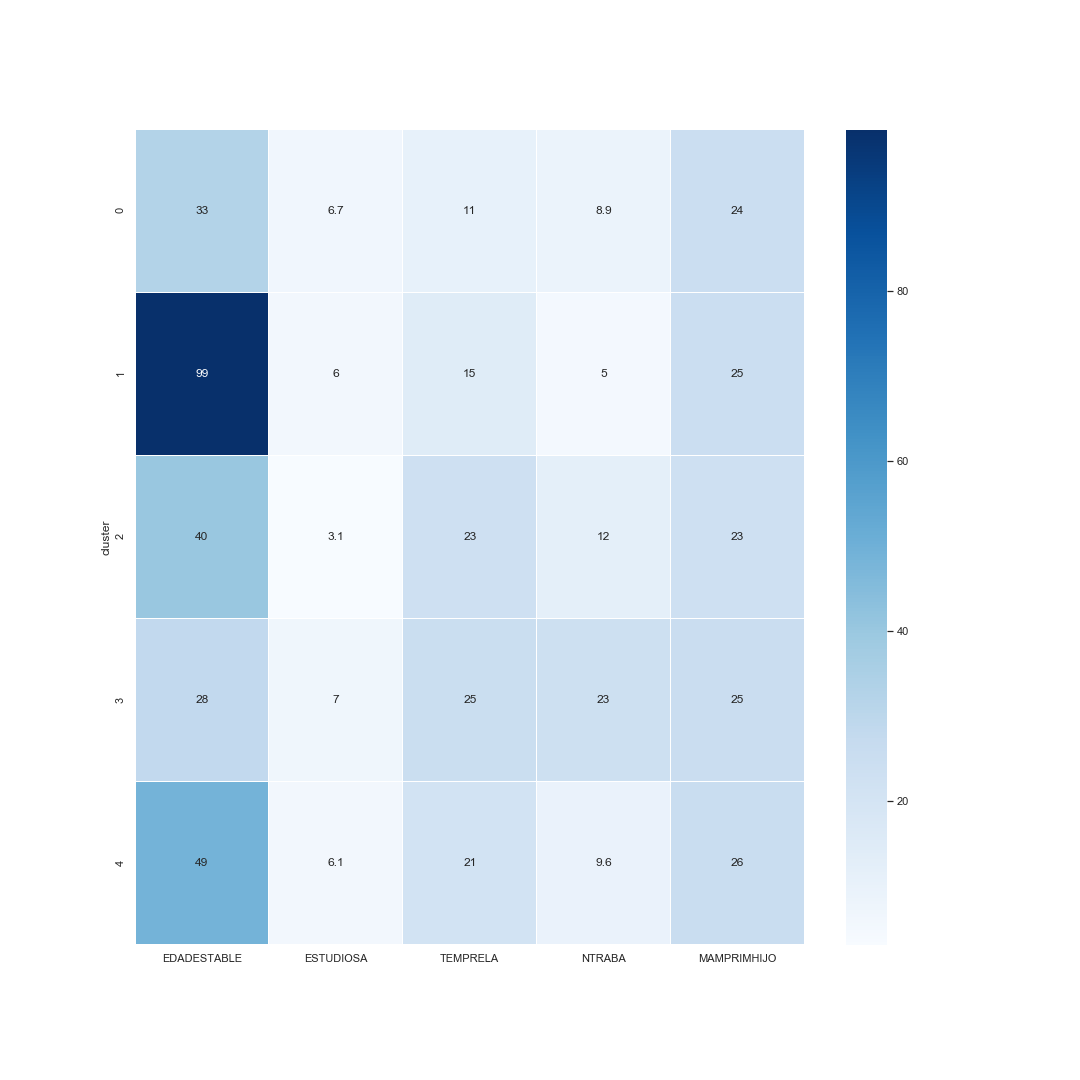
\includegraphics[width=0.56\textwidth]{../img/heatmap/Caso1-AgglomerativeClustering.png}}
		\subfloat[DBSCAN]{
			\label{f:DBSCAN}
			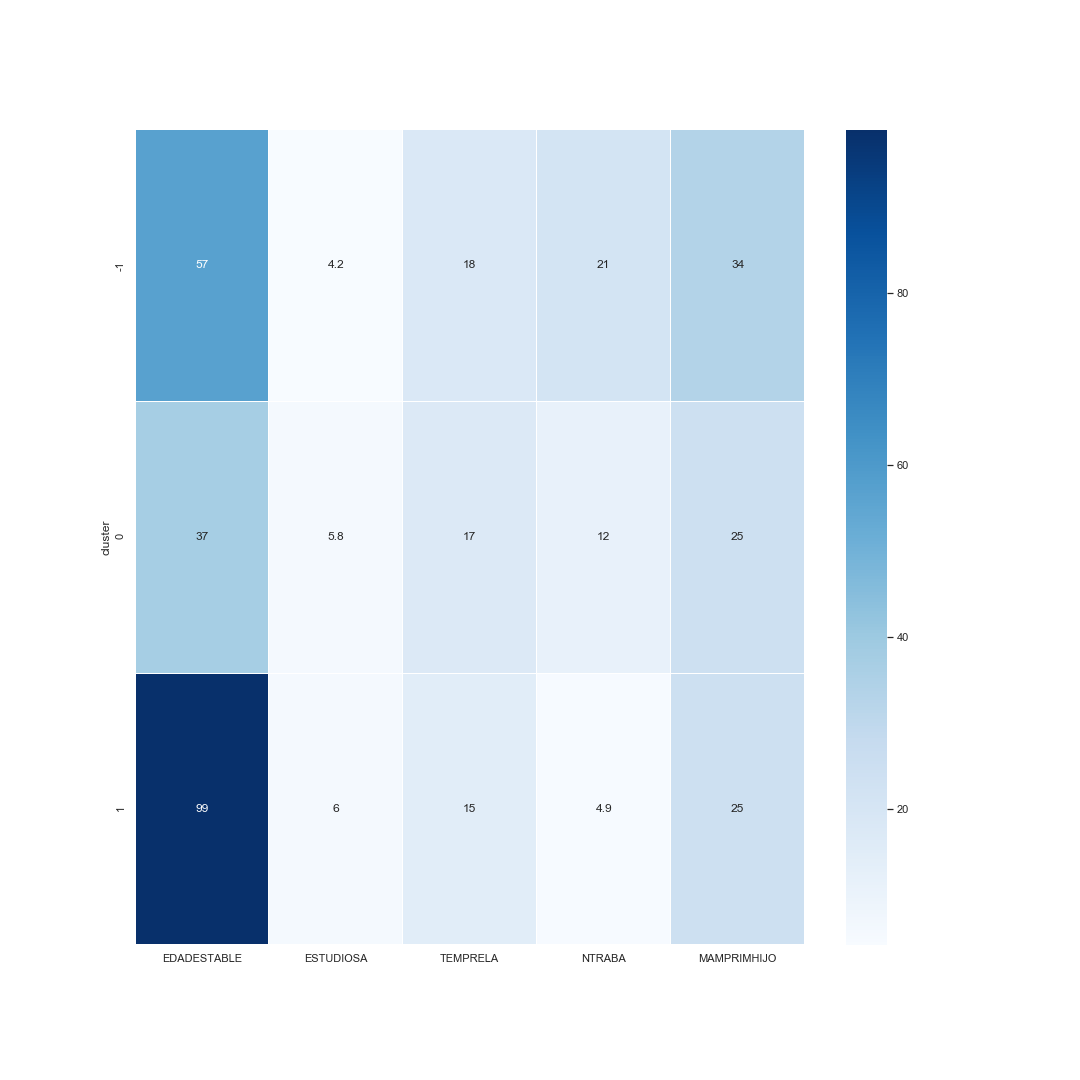
\includegraphics[width=0.56\textwidth]{../img/heatmap/Caso1-DBSCAN.png}}
		
	\end{figure}
	
	
	\begin{figure}[H]
		\centering
		
		\subfloat[MiniBatchKM]{
			\label{f:MiniBatchKM}
			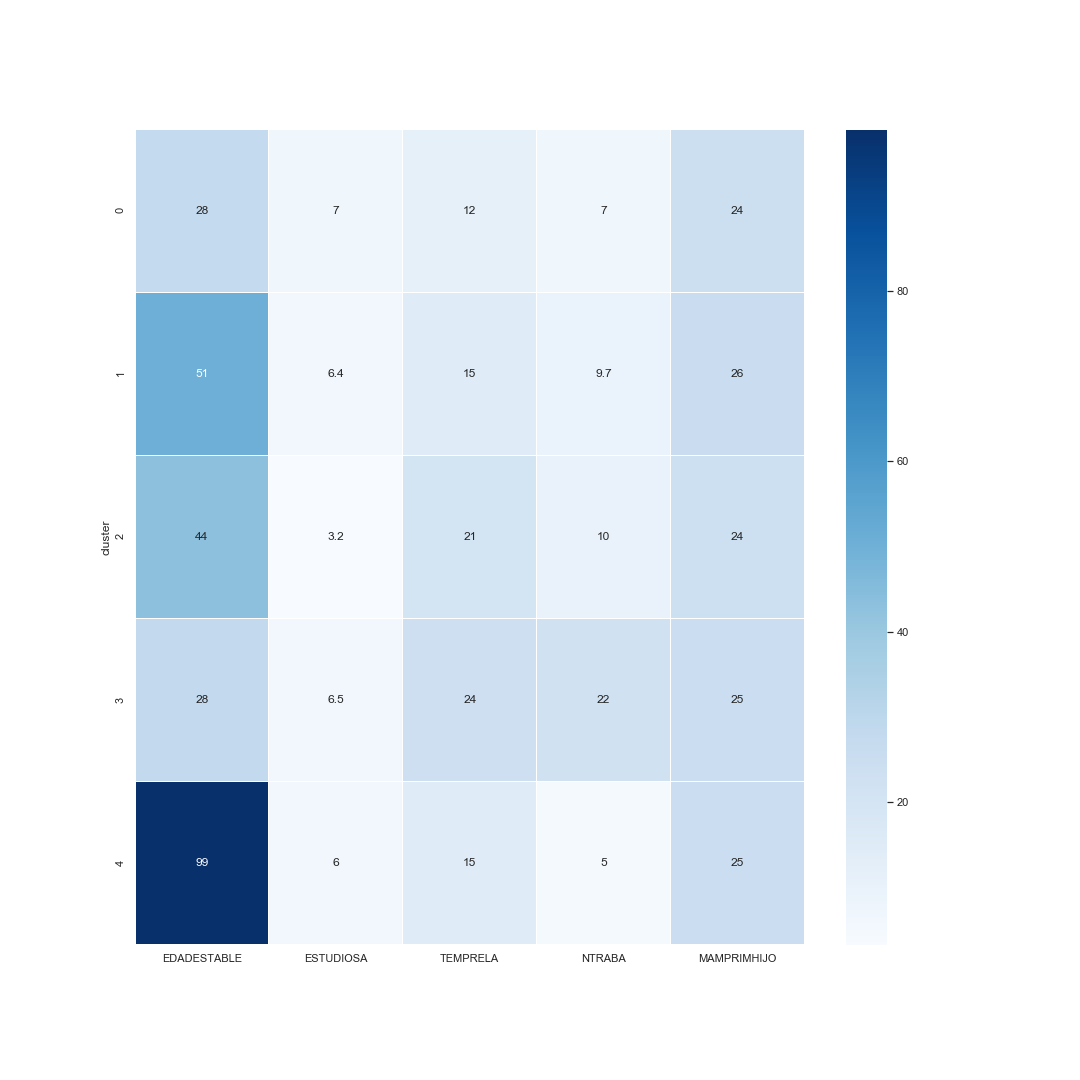
\includegraphics[width=0.56\textwidth]{../img/heatmap/Caso1-MiniBatchKM.png}}
		\subfloat[KMeans]{
			\label{f:KMeans}
			\includegraphics[width=0.56\textwidth]{../img/heatmap/Caso1-KMeans.png}}
		
		
	\end{figure}


	\begin{figure}[H]
		\centering
		\subfloat[MeanShift]{
			\label{f:MeanShift}
			\includegraphics[width=0.7\textwidth]{../img/heatmap/Caso1-MeanShift.png}}
		
	\end{figure}
	
	Observando el heatmap de \texttt{AgglomerativeClustering}, se nos va la vista al valor 99 de \texttt{EDADESTABLE} en el cluster 1. Con alta proporción este valor es un error ya que no tiene sentido que se obtenga un trabajo estable a la edad de 99 años, por esto es de vital importancia estudiar y contrastar los datos. \\
	En este caso obviamos esta región para no arrastrar posibles errores en la explicación. Además, en los futuros gráficos kplot y boxplot, dicha región estará alterada.\\
	
	En una visión general, observamos que en el cluster 0 y 3, existe una relación entre el nivel de estudios alcanzado (\texttt{ESTUDIOSA}) y la edad a la que se obtuvo el primer trabajo estable. Vemos que con un título universitario cercano al valor 7, se obtiene un trabajo estable (\texttt{EDADESTABLE}) más temprano. \\
	
	Por otro lado, la variable \texttt{MAMPRIMHIJO} no infiere en el resto de variables. \texttt{TEMPRELA} tampoco. \\
	
	Observando el resto de Heatmaps, vemos que sigue el valor de 99 años como edad a la que obtuvo su trabajo estable, además, la variable \texttt{MAMPRIMHIJO} no influye en el resto de variables pues se mantiene estable.
	
	





	\subsection{Dendogram}
	
	Mostramos el dendograma del algoritmo \texttt{AgglomerativeClustering}, un árbol de clúster donde cada grupo está vinculado a dos o más grupos de sucesores. Estos grupos están anidados y organizados como un árbol.
	
	Mostramos los resultados obtenidos:
	\begin{figure}[H]
		\centering
		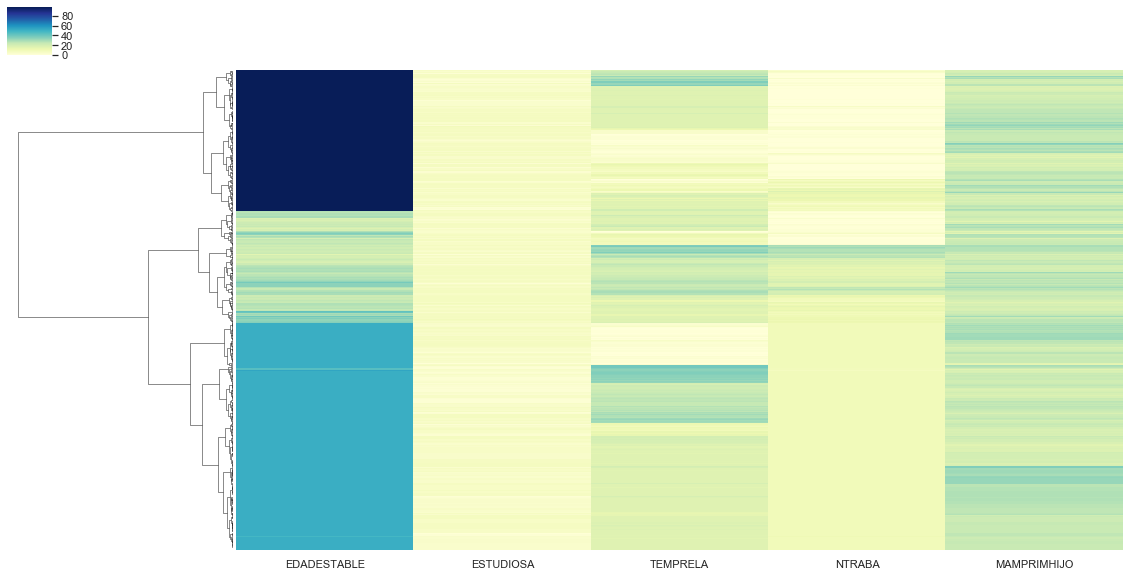
\includegraphics[scale=0.3]{../img/dendogram/Caso1-AgglomerativeClustering.png}
		
		\caption{Dendogram}
	\end{figure}


	Hemos modificado ligeramente el código para obtener un dendograma más completo.
	
	
	
	
	
	
	\subsection{ScatterMatrix}
	
	Un \texttt{Scatter Matrix} es una colección de scatterplots organizadas en una matriz. Cada región (scatterplot), representa la relación que existe entre el par de variables. Puede ser usado para determinar el grado de correlación entre las variables.
	
	\newpage
	Mostramos los resultados obtenidos tras ejecutar los 5 algoritmos:
	
	\begin{figure}[H]
		\centering
		\subfloat[Agglo]{
			\label{f:Agglo}
			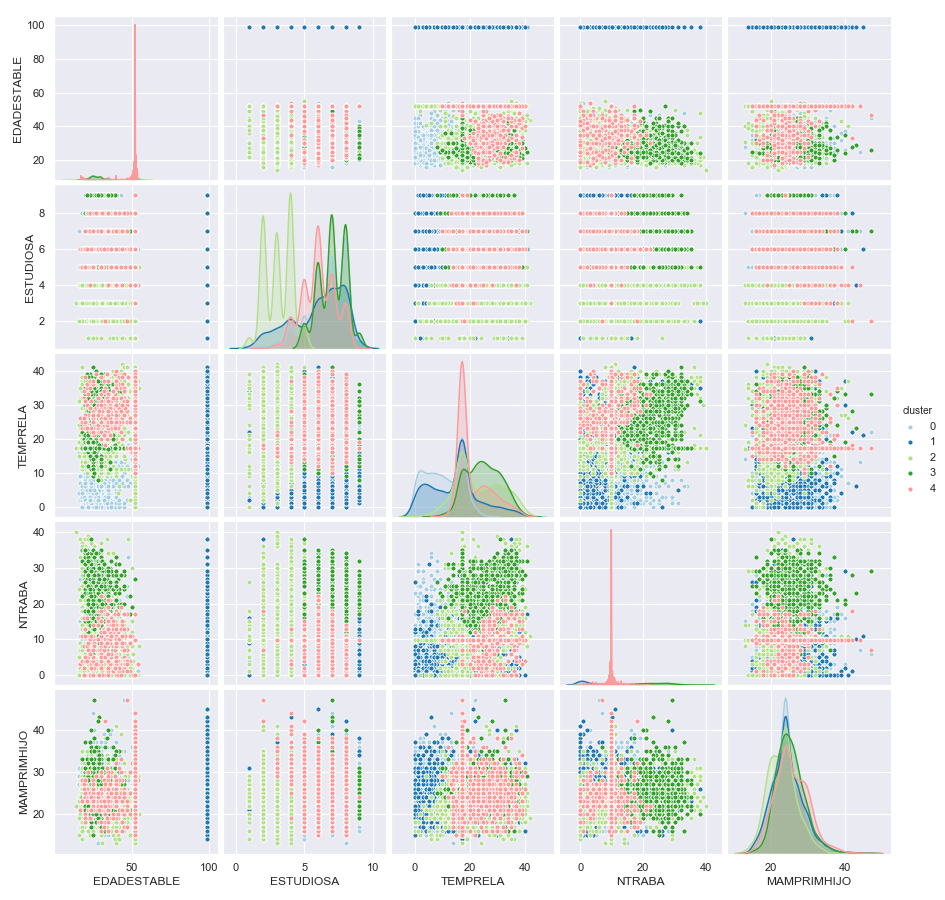
\includegraphics[width=0.55\textwidth]{../img/scatter/Caso1-AgglomerativeClustering.png}}
		\subfloat[DBSCAN]{
			\label{f:DBSCAN}
			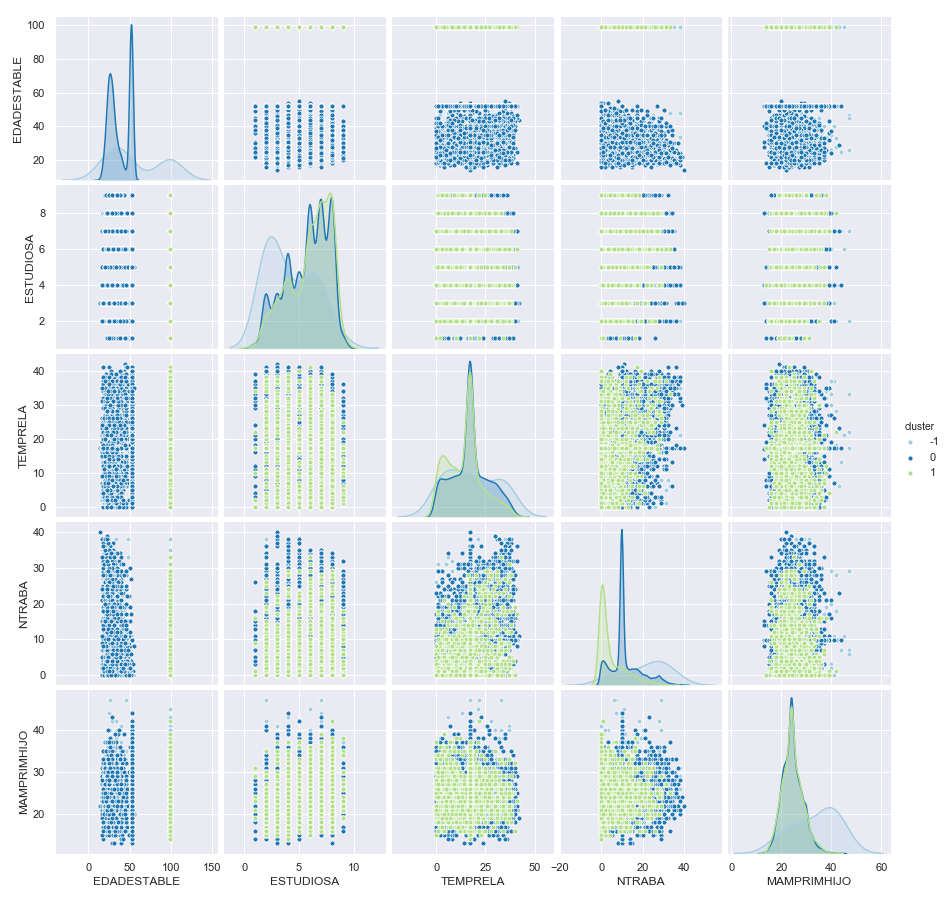
\includegraphics[width=0.55\textwidth]{../img/scatter/Caso1-DBSCAN.png}}
		
	\end{figure}
	
	
	\begin{figure}[H]
		\centering
		
		\subfloat[MiniBatchKM]{
			\label{f:MiniBatchKM}
			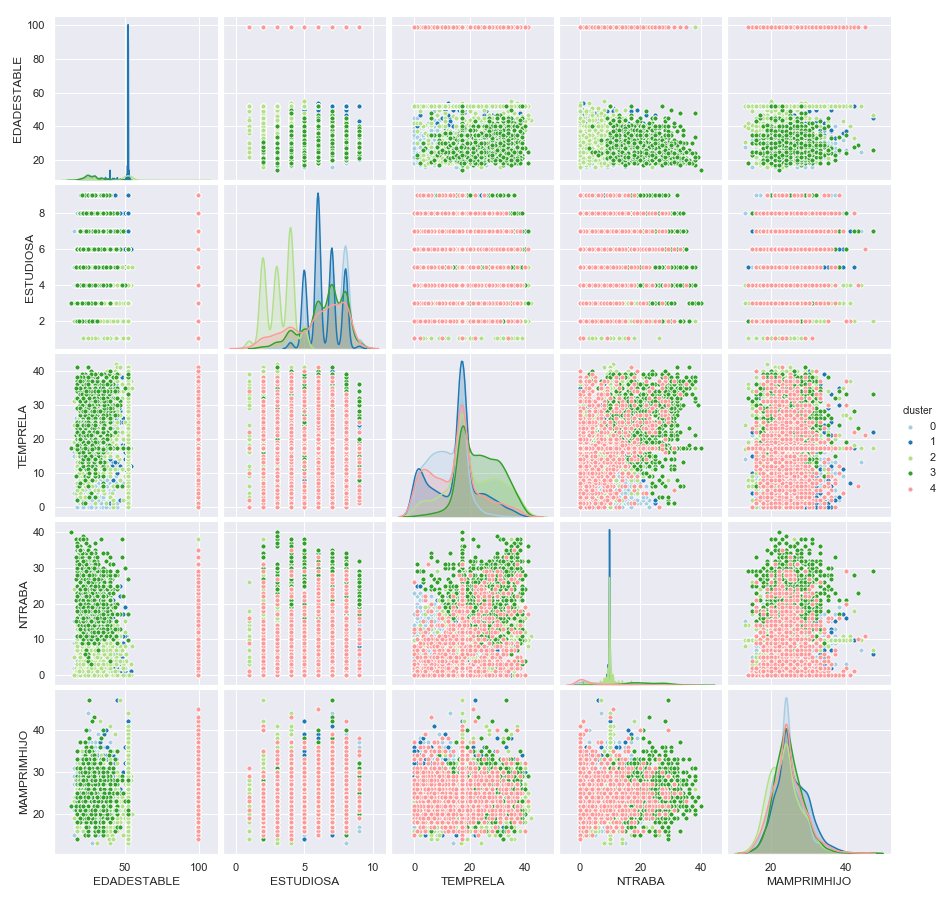
\includegraphics[width=0.55\textwidth]{../img/scatter/Caso1-MiniBatchKM.png}}
		\subfloat[KMeans]{
			\label{f:KMeans}
			\includegraphics[width=0.55\textwidth]{../img/scatter/Caso1-KMeans.png}}
		
		
	\end{figure}
	
	
	\begin{figure}[H]
		\centering
		\subfloat[MeanShift]{
			\label{f:MeanShift}
			\includegraphics[width=0.6\textwidth]{../img/scatter/Caso1-MeanShift.png}}
		
	\end{figure}
	
	
	
	\subsection{Kplot y BoxPlot}
	
	Existen otros gráficos que nos permiten visualizar nuestros casos de estudio:
	\begin{itemize}
		\item \texttt{Kplot}: Se trata de un diagrama de densidad. Visualiza la distribución de los datos en su intervalo correspondiente. Una de sus ventajas es que determinan la forma de la distribución, independientemente del número de \textit{bins}. El eje \textbf{X} representa el rango de valores que toma la variable y el eje \textbf{Y}, la densidad.
		
		
		\begin{figure}[H]
			\centering
			\subfloat[Kmeans - Kplot]{
				\label{f:Kmeans}
				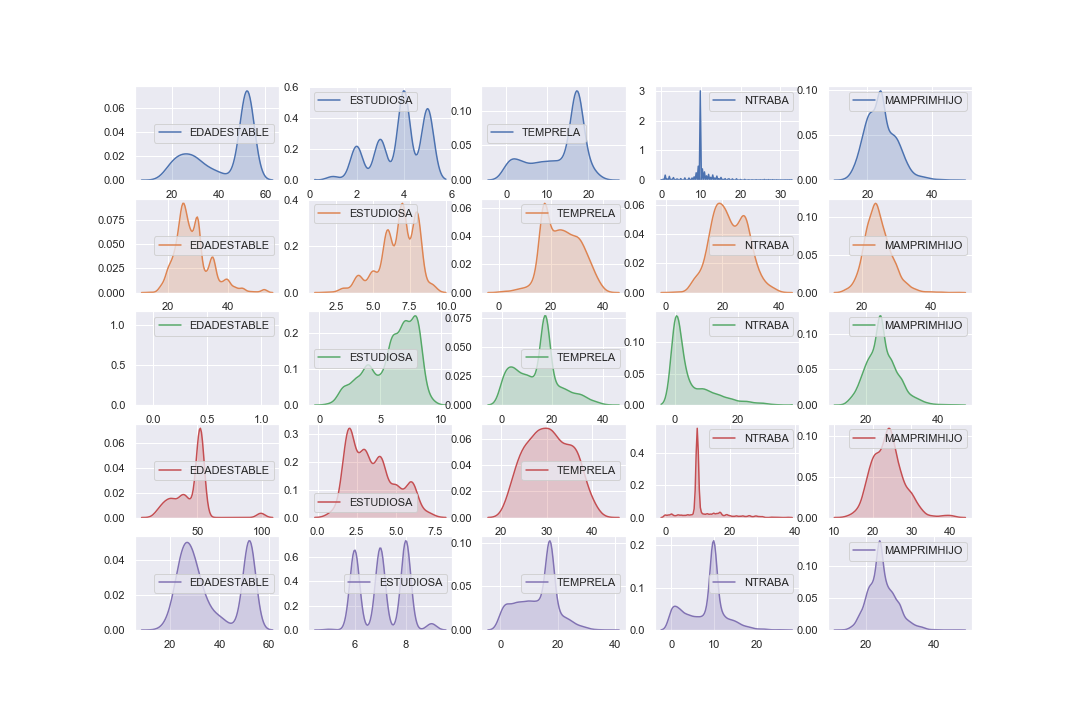
\includegraphics[width=0.94\textwidth]{../img/kplot/KMeans_1Kplot.png}}
			
		\end{figure}
	
	
	
		\item \texttt{BoxPlot}: También llamado diagrama de caja. Es un método estandarizado para representar gráficamente una seria de datos numéricos a través de sus cuartiles. De esta forma, el diagrama de caja muestra a simple vista la mediana y los cuartiles de los datos, pudiendo también representar los valores atípicos de estos.
		
		Mostramos únicamente el generado por \texttt{Kmeans}. El resto de diagramas están en la carpeta de imágenes entregada en la práctica.
		
		\begin{figure}[H]
			\centering
			\subfloat[Kmeans - BoxPlot]{
				\label{f:Kmeans}
				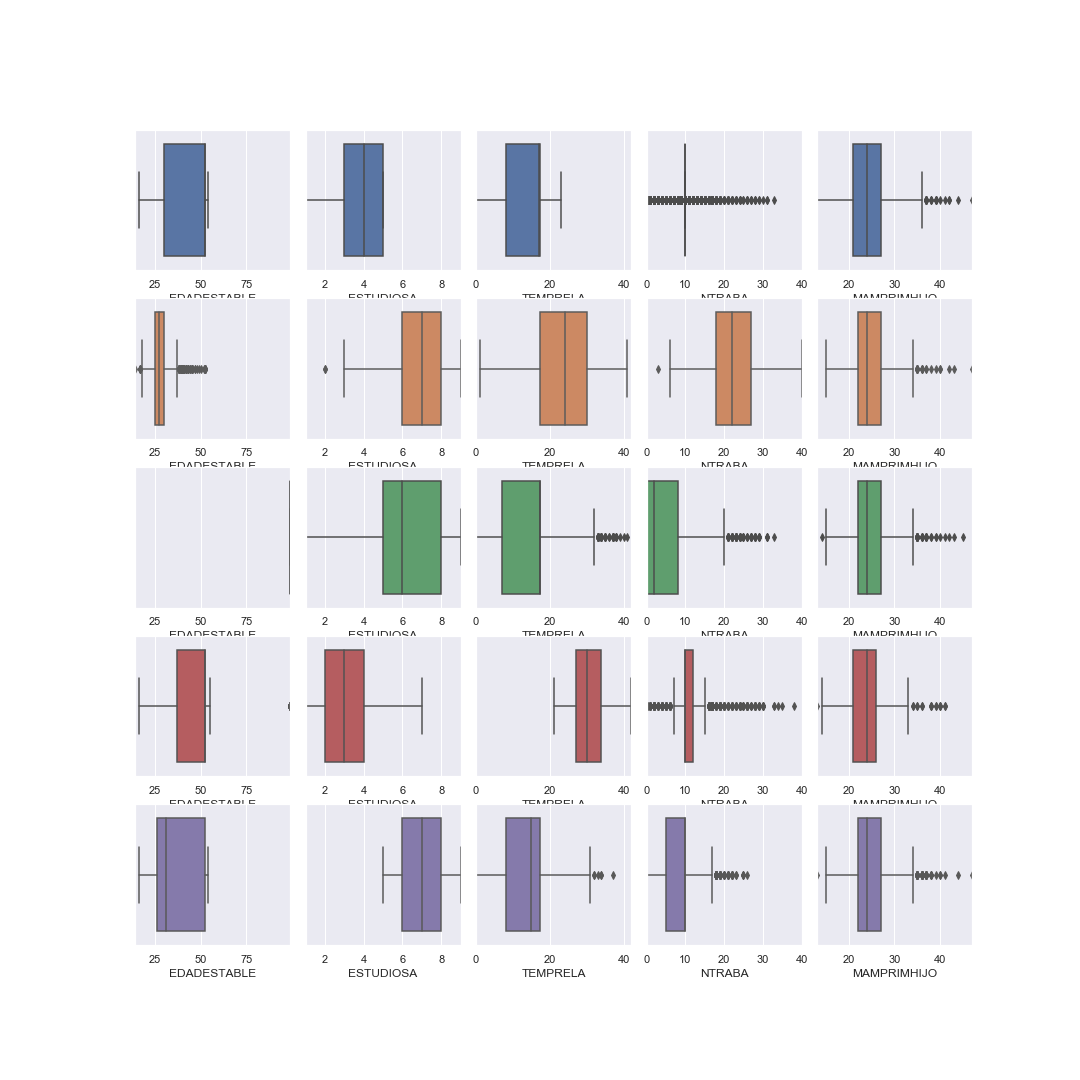
\includegraphics[width=1\textwidth]{../img/boxplot/KMeans_1boxplot.png}}
			
		\end{figure}
	\end{itemize}
	
	
	\newpage
	
	\subsection{Interpretación de la segmentación}
	
	En el fichero generado \textit{caso\_1.txt} se han volcado los resultados obtenidos, entre los cuales se han calculado:
	
	\begin{itemize}
		\item \texttt{Tamaño de la muestra}: En el caso 1, el tamaño ha sido de 8181.
		\item Para cada algoritmo se ha calculado el \texttt{tamaño de cada cluster}		
		\item \texttt{Resultados}: Tabla comparativa de los resultados finales de todos los algoritmos, las métricas y el tiempo de ejecución.
		
		\begin{table}[H]

				\begin{tabular}{|l|l|l|l|l|}
					\hline
					\textbf{Algoritmo}               & \textbf{Clusters} & \textbf{SH} & \textbf{SC} & \textbf{Tiempo} \\ \hline
					\textbf{KMeans}                  & 5                 & 0.268672    & 3152.287047 & 0.453316        \\ \hline
					\textbf{AgglomerativeClustering} & 5                 & 0.209059    & 2801.905883 & 8.399320        \\ \hline
					\textbf{MeanShift}               & 2                 & 0.402552    & 4034.626526 & 22.283585       \\ \hline
					\textbf{MiniBatchKM}             & 5                 & 0.240193    & 3036.829553 & 0.165094        \\ \hline
					\textbf{DBSCAN}                  & 3                 & 0.361889    & 2032.787376 & 2.702886        \\ \hline
				\end{tabular}%
			
		\end{table}
	
	
	
	
	
	El algoritmo que muestra mejor valor de las métricas es \texttt{MeanShift}, sin embargo tiene un tiempo de ejecución bastante mayor, casi unas 20 veces más. Observando el algoritmo \texttt{Kmeans}, vemos que tiene unos índices relativamente buenos y su tiempo de ejecución es muy bajo. Por otro lado, \texttt{MiniBatchKmeans} empeora los resultados de los índices de \texttt{Kmeans} pero mejora el tiempo de ejecución. \\
	
	
	\end{itemize}
	
	
	
	
	Mostramos el tamaño de cada cluster para el mejor algoritmo, \texttt{MeanShift}:
	
	\begin{table}[H]
	\centering
			\begin{tabular}{|l|l|}
				\hline
				\textbf{Cluster} & \textbf{Tamaño de cada cluster} \\ \hline
				0:               & 6677 (81.62\%)                  \\ \hline
				1:               & 1504 (18.38\%)                  \\ \hline
			\end{tabular}%
		
	\end{table}

	La proporción de muestras se distribuye de forma diferente. En el primer cluster se concentra un 81\% de la muestra mientras que en el segundo un 18\%. Realmente, hay suficientes datos en el segundo cluster para sacar resultados fiables, pero no mayores que en el primero ya que al tener más encuestas, se pueden sacar conclusiones más fiables.
	
	
	\subsubsection{Modificaciones}
	
	En relación a las modificaciones pedidas, estudiaremos la variación de los algoritmos \texttt{KMean} y \texttt{Agglomerative}. El primero es el que se pedía en la práctica como uso obligatorio y el segundo me ha parecido buena idea ya que es el único algoritmo jerárquico que he usado.
	
	
	\begin{lstlisting}[frame=single]
wardAgglo_5=AgglomerativeClustering(n_clusters=5,linkage='ward')
wardAgglo_2=AgglomerativeClustering(n_clusters=2,linkage='ward')
	
k_means_5 = KMeans(init='k-means++', n_clusters=5, n_init=5,
			random_state=random_seed)
k_means_2 = KMeans(init='k-means++', n_clusters=2, n_init=5, 
			random_state=random_seed)
	
modificacion = [("Agglo_5", wardAgglo_5),
("Agglo_2", wardAgglo_2),
("KMeans_5", k_means_5),
("KMeans_2", k_means_2)]
	
ClusteringAlgorithms(modificacion, X1, X1_normal, 4, usadas1)
ClusteringAlgorithms(modificacion, X2, X2_normal, 5, usadas2)
ClusteringAlgorithms(modificacion, X3, X3_normal, 6, usadas3)
	\end{lstlisting}
	
	
	
	
	
	
	
	
	Para ambos estudiaremos los índices \texttt{Silhouette} y \texttt{Calinski Harabaz}, con 2 y 5 clusters y para los tres casos de estudio.
	Pensamos que un menor número de clusters se reflejará en mejores índices de las métricas anteriores ya que los datos no estarán divididos tan desproporcionalmente que si tuvieran más clusters.
	
	Para el caso 1, tenemos:
	\begin{itemize}
		\item Tamaño de los clusters
		
		\begin{table}[H]
		\centering
				\begin{tabular}{|l|l|l|l|l|}
					\cline{1-2} \cline{4-5}
					\textbf{Agglo5} & \textbf{Tamaño de cluster} & \multirow{6}{*}{} & \textbf{Kmean5} & \textbf{Tamaño de cluster} \\ \cline{1-2} \cline{4-5} 
					0:              & 2959 (36.17\%)             &                   & 4:              & 2931 (35.83\%)             \\ \cline{1-2} \cline{4-5} 
					2:              & 1582 (19.34\%)             &                   & 0:              & 1596 (19.51\%)             \\ \cline{1-2} \cline{4-5} 
					1:              & 1504 (18.38\%)             &                   & 2:              & 1480 (18.09\%)             \\ \cline{1-2} \cline{4-5} 
					4:              & 1313 (16.05\%)             &                   & 1:              & 1254 (15.33\%)             \\ \cline{1-2} \cline{4-5} 
					3:              & 823 (10.06\%)              &                   & 3:              & 920 (11.25\%)              \\ \cline{1-2} \cline{4-5} 
				\end{tabular}%
			
		\end{table}
	
	
		\begin{table}[H]
		\centering
				\begin{tabular}{|l|l|l|l|l|}
					\cline{1-2} \cline{4-5}
					\textbf{Agglo2} & \textbf{Tamaño de cluster} &  & \textbf{Kmean2} & \textbf{Tamaño de cluster} \\ \cline{1-2} \cline{4-5} 
					0:              & 6677 (81.62\%)             &  & 0:              & 6677 (81.62\%)             \\ \cline{1-2} \cline{4-5} 
					1:              & 1504 (18.38\%)             &  & 1:              & 1504 (18.38\%)             \\ \cline{1-2} \cline{4-5} 
				\end{tabular}%
			
		\end{table}
	
		Como hemos comentado anteriormente, el hecho de tener un mayor número de clusters hace que los datos se tengan que dividir en estos y así se producen porcentajes desproporcionales.
	
	
		\item Resultados obtenidos:
		
		\begin{table}[H]
				\centering
				\begin{tabular}{|l|l|l|l|l|}
					\hline
					\textbf{Algoritmo} & \textbf{Número Clusters} & \textbf{SH} & \textbf{CH} & \textbf{Tiempo} \\ \hline
					Agglo\_5           & 5                        & 0.209059    & 2801.905883 & 8.263324        \\ \hline
					Agglo\_2           & 2                        & 0.402552    & 4034.626526 & 8.294797        \\ \hline
					KMeans\_5          & 5                        & 0.268672    & 3152.287047 & 0.406277        \\ \hline
					KMeans\_2          & 2                        & 0.402552    & 4034.626526 & 0.234406        \\ \hline
				\end{tabular}%
			
		\end{table}
	
		Vemos la tabla creada tras realizar la ejecución. El tiempo de ejecución en el algoritmo jerárquico \texttt{Agglomerative Clustering} es mayor que en \texttt{Kmeans}, además, observando este último, con 5 clusters tarda el doble que con 2. Observando los resultados de las métricas, sucede lo que hemos predecido, los algoritmos con 2 clusters obtienen mejores resultados que los algoritmos con 5, ¡Casi el doble!


	\end{itemize}
	
	
	
	
	
	
	
	
	
	
	
	
	
	
	\section{Caso de estudio 2}
	
	Escogemos el grupo de mujeres jóvenes (menores de 40 años) cuyo anticonceptivo más usado no es el preservativo, es decir, que hayan usado métodos anticonceptivos hormonales, DIU de cobre...etc. 
	
	
	\begin{lstlisting}[frame=single][language=Python]
subset = datos.loc[(datos['EDAD']<40) &
 (datos['MODAANTICONCEP']!=5) & (datos['MODAANTICONCEP']!=14)]
usadas=['PRACTICANTE','NEMBANT','NHIJOBIO','NPARANT','NDESEOHIJO']
	\end{lstlisting}
	
	
	Explicamos la variables usadas:
	\begin{itemize}
		\item \texttt{PRACTICANTE}: Cómo de practicante se considera el entrevistado. Varía desde 1 (poco practicante) hasta 6 (muy practicante). 
		\item \texttt{NEMBANT}: Número de embarazos anteriores.
		\item \texttt{NHIJOBIO}: Número de hijos biológicos.
		\item \texttt{NPARANT}: Número de exparejas con las que ha convivido.
		\item \texttt{NDESEOHIJO}: Número de hijos deseados para los que tienen hijos y los que no.
	\end{itemize}
	
	Hemos escogido el grupo de entrevistadas que han usado anticonceptivos diferentes al preservativo. Queremos ver si esto se relaciona con el nivel de religiosidad y en general, con los hijos que tiene o ha querido tener.
	
	
	
	\subsection{Heatmap}
	Mostramos los diferentes heatmaps o mapas de calor de los algoritmos:
	
	\begin{figure}[H]
		\centering
		\subfloat[Agglo]{
			\label{f:Agglo}
			\includegraphics[width=0.55\textwidth]{../img/heatmap/Caso2-AgglomerativeClustering.png}}
		\subfloat[DBSCAN]{
			\label{f:DBSCAN}
			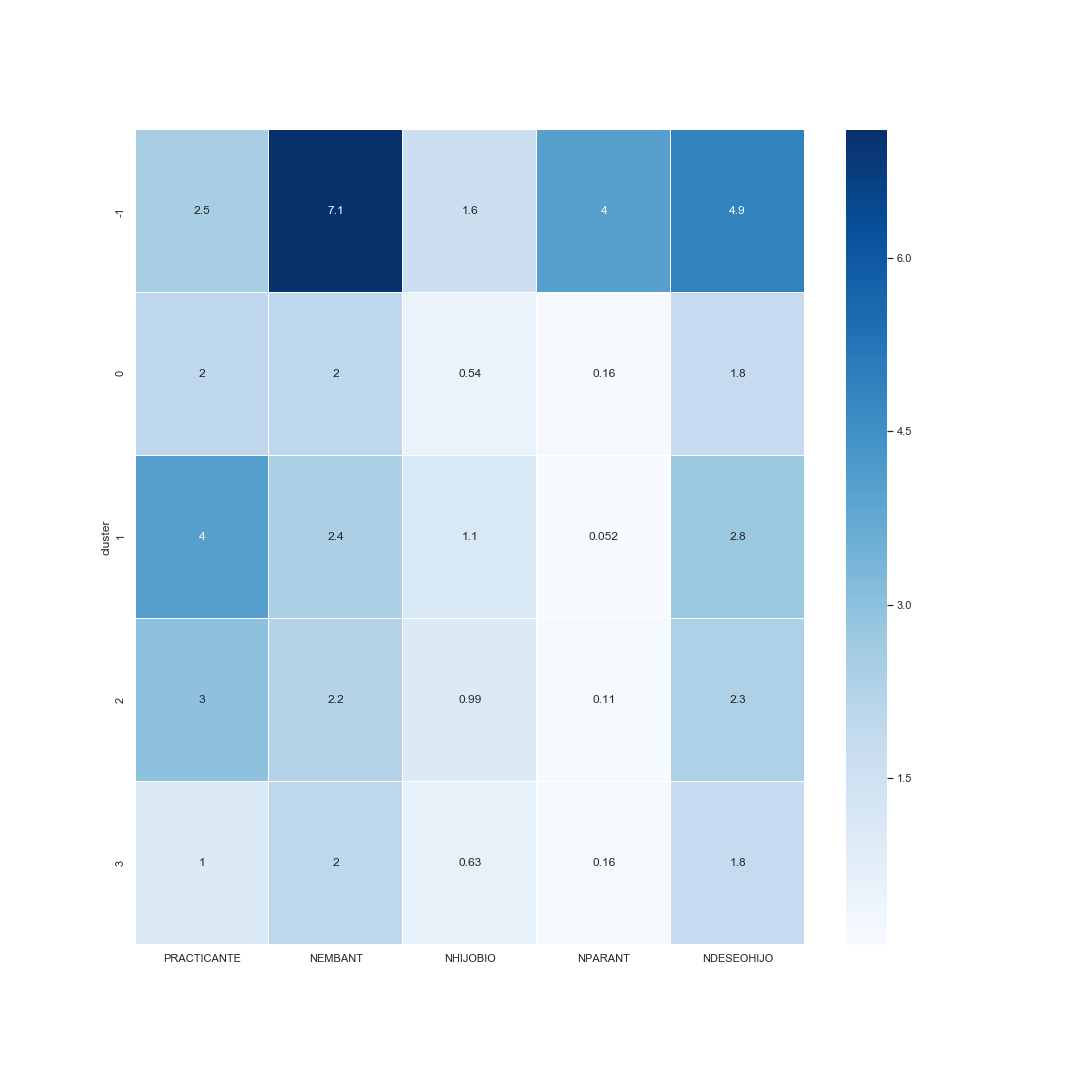
\includegraphics[width=0.55\textwidth]{../img/heatmap/Caso2-DBSCAN.png}}
		
	\end{figure}
	
	
	\begin{figure}[H]
		\centering
		
		\subfloat[MiniBatchKM]{
			\label{f:MiniBatchKM}
			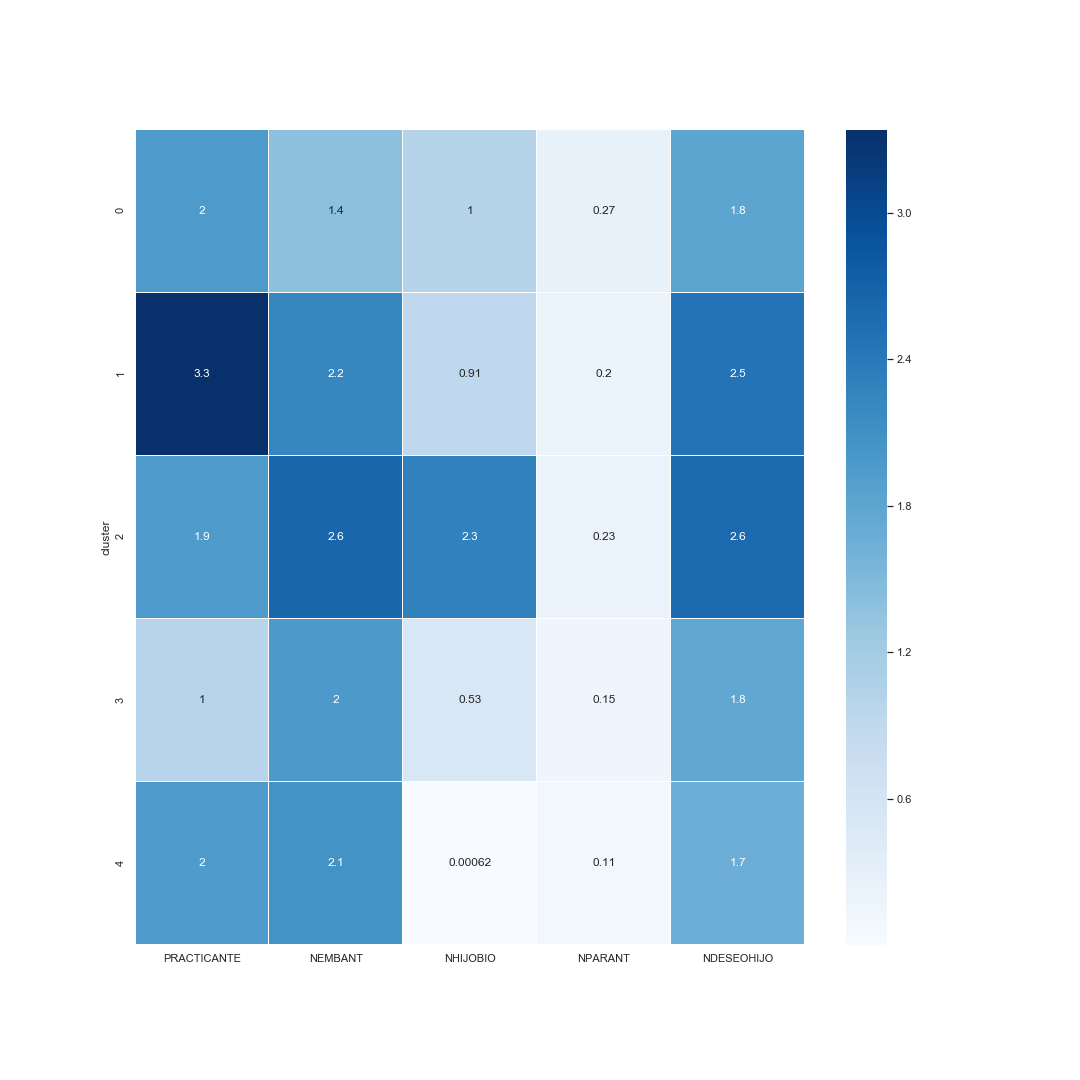
\includegraphics[width=0.6\textwidth]{../img/heatmap/Caso2-MiniBatchKM.png}}
		\subfloat[KMeans]{
			\label{f:KMeans}
			\includegraphics[width=0.6\textwidth]{../img/heatmap/Caso2-KMeans.png}}
		
		
	\end{figure}
	
	
	\begin{figure}[H]
		\centering
		\subfloat[MeanShift]{
			\label{f:MeanShift}
			\includegraphics[width=0.7\textwidth]{../img/heatmap/Caso2-MeanShift.png}}
		
	\end{figure}

	Como vemos y era de esperar, observando \texttt{Agglomerative Clustering} Las entrevistadas no son muy practicantes ya que hay tres clusters que se mantienen con un nivel inferior a la mitad y otros dos con un valor de 3.3 sobre 4 (recordemos que el máximo nivel de práctica era este). \\ 
	
	
	El número de embarazo aumenta ligeramente a mayor nivel de religiosidad, así como el número de hijos biológicos y los deseados ya que las zonas más intensas de color están en los cluster 2 y 4. 
	Por otro lado, el número de exparejas no aporta apenas información relevante. \\
	
	Observamos ahora \texttt{MiniBatchKM}. En este caso, vemos que ocurre exactamente lo mismo. Por ejemplo, en el cluster 1 y 2 (mayores niveles de religiosidad obtenidos), vemos que el número de embarazos y el número deseado de hijos son directamente proporcionales. \\
	
	Por último, estudiamos \texttt{Meanshift} y todos los clusters permitidos (como hemos explicado anteriormente).
	En este caso no sacamos conclusiones realmente relevantes. Vemos que en el cluster 9 el número de exparejas (37) se relaciona con un mayor número de hijos deseados, 16. 

	\subsection{Dendogram}
	
	A continuación, mostramos el dendograma, que es la forma de representar el clustering jerárquico usado en el algoritmo \texttt{Agglomerative Clustering}
	
	\begin{figure}[H]
		\centering
		\includegraphics[scale=0.37]{../img/dendogram/Caso2-AgglomerativeClustering.png}
		
		\caption{Dendogram}
	\end{figure}





	\newpage
	\subsection{ScatterMatrix}
	
	Por último, mostramos los Scatter Matrix obtenidos tras la ejecución y observar así la correlación de las variables:
	
	\begin{figure}[H]
		\centering
		\subfloat[Agglo]{
			\label{f:Agglo}
			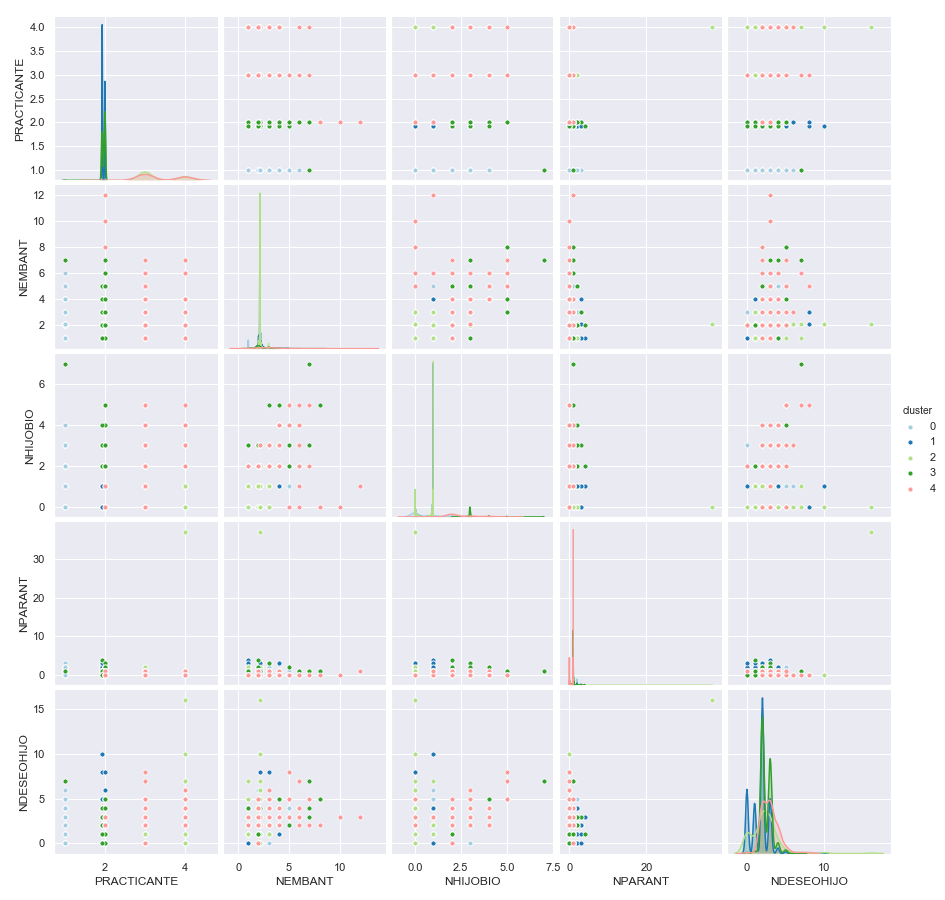
\includegraphics[width=0.55\textwidth]{../img/scatter/Caso2-AgglomerativeClustering.png}}
		\subfloat[DBSCAN]{
			\label{f:DBSCAN}
			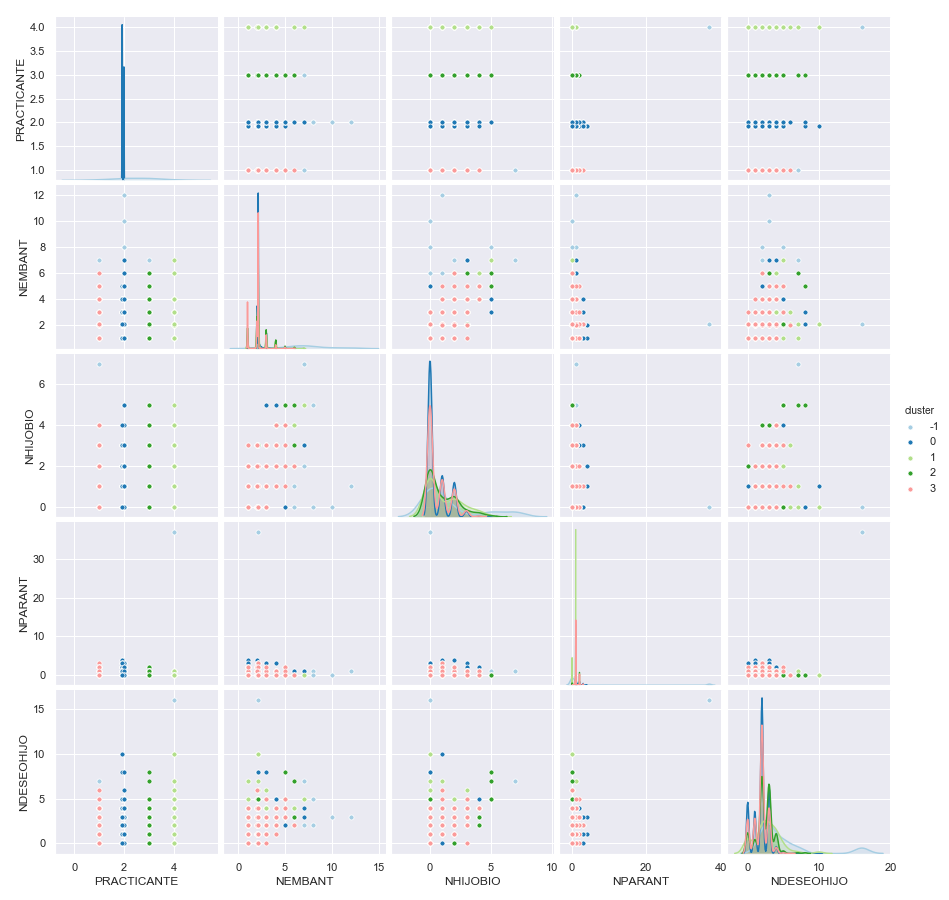
\includegraphics[width=0.55\textwidth]{../img/scatter/Caso2-DBSCAN.png}}
		
	\end{figure}
	
	
	\begin{figure}[H]
		\centering
		
		\subfloat[MiniBatchKM]{
			\label{f:MiniBatchKM}
			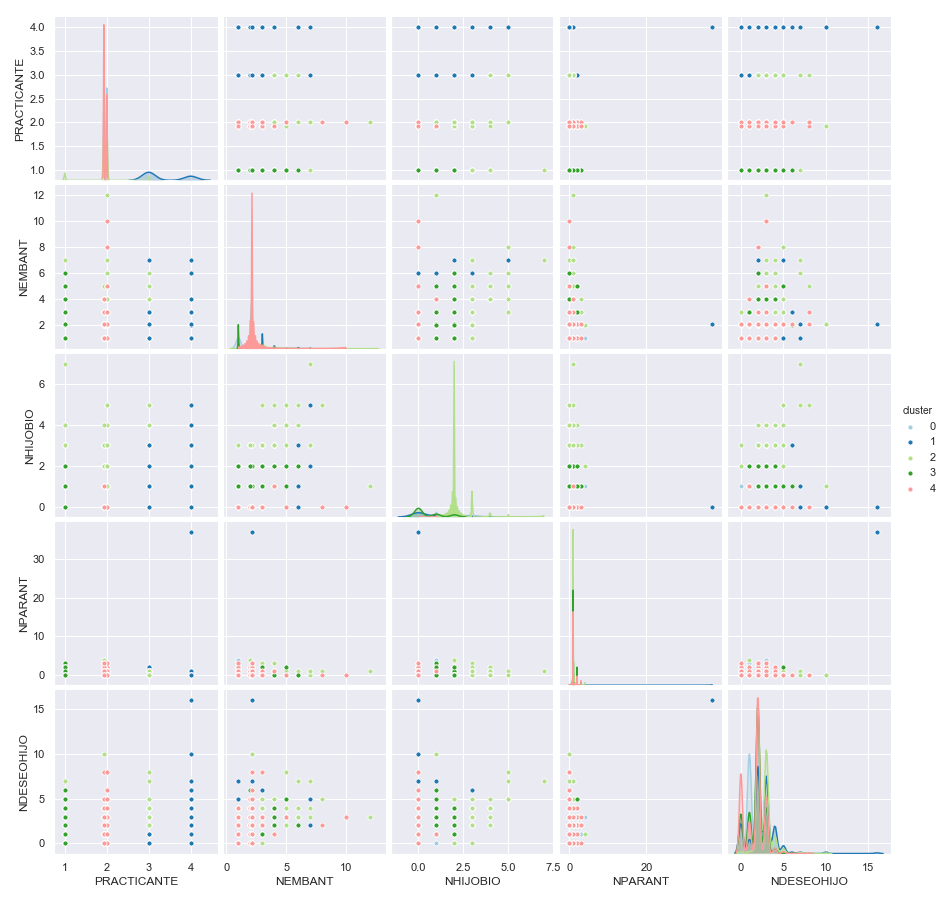
\includegraphics[width=0.55\textwidth]{../img/scatter/Caso2-MiniBatchKM.png}}
		\subfloat[KMeans]{
			\label{f:KMeans}
			\includegraphics[width=0.55\textwidth]{../img/scatter/Caso2-KMeans.png}}
		
		
	\end{figure}
	
	
	\begin{figure}[H]
		\centering
		\subfloat[MeanShift]{
			\label{f:MeanShift}
			\includegraphics[width=0.57\textwidth]{../img/scatter/Caso2-MeanShift.png}}
		
	\end{figure}



	\subsection{Kplot y BoxPlot}
	
	Ahora bien, mostramos la gráfica de densidad KPlot y el diagrama de caja \texttt{BoxPlot}.
	
	\begin{itemize}
		\item \texttt{KPlot}: Con una vista rápida, podemos ver que los datos están centrados y no a los extremos de los intervalos.  Recordemos también que el eje \texttt{X} representa el intervalo de la variable y el eje \texttt{Y} la densidad.
		
		
		\begin{figure}[H]
			\centering
			\subfloat[Kmeans - KPlot]{
				\label{f:Kmeans}
				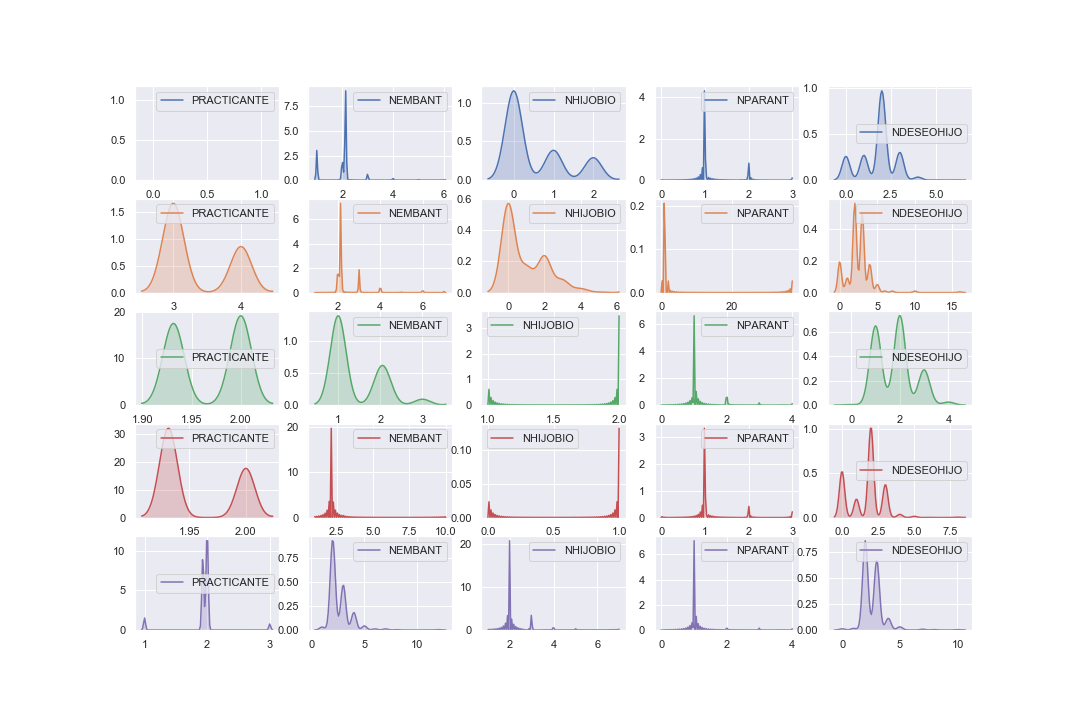
\includegraphics[width=1.06\textwidth]{../img/kplot/KMeans_2Kplot.png}}
			
		\end{figure}
	
	
		\item \texttt{BoxPlot}: Mostramos ahora el diagrama de cajas obtenido con el algoritmo Kmeans.
		
		
		
		\begin{figure}[H]
			\centering
			\subfloat[Kmeans - BoxPlot]{
				\label{f:Kmeans}
				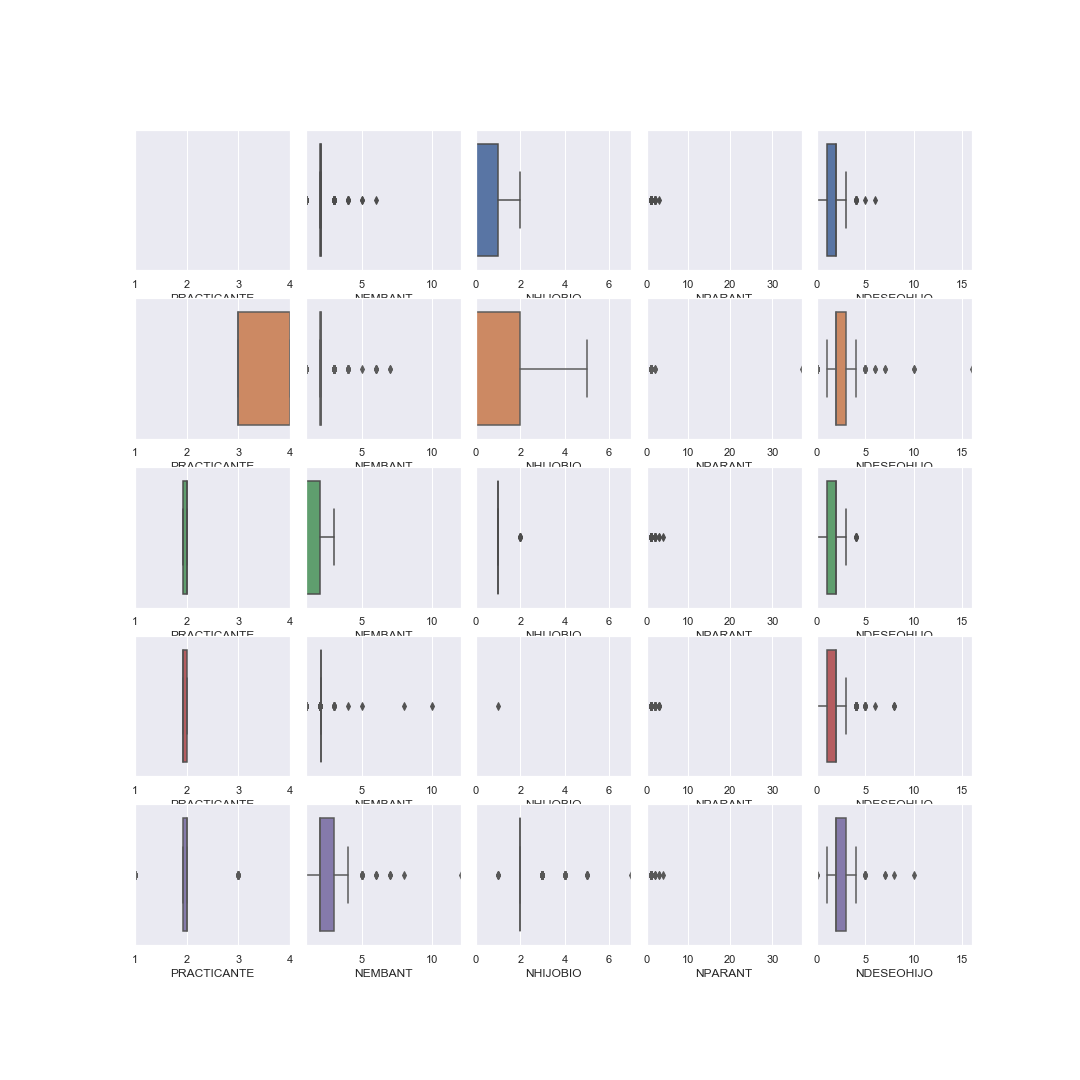
\includegraphics[width=0.85\textwidth]{../img/boxplot/KMeans_2boxplot.png}}
			
		\end{figure}
	\end{itemize}
	





	\subsection{Interpretación de la segmentación}
	
	Volvemos a volcar los datos en el fichero de texto \texttt{caso\_2.txt}.
	
	
	\begin{itemize}
		\item El tamaño de la muestra en este caso es de 3456 instancias.
		\item Para cada algoritmo se ha creado en el fichero una tabla con el tamaño de cada cluster (no se ponen aquí por redundancia)
		
		\item Se han calculado para todos los algoritmos las dos métricas anteriormente explicadas, \texttt{Silhoutte y Calinski Harabasz}
		
		\item Por último, mostramos una tabla comparativa:
	\end{itemize}
	
	
	\begin{table}[H]
		\resizebox{\textwidth}{!}{%
			\begin{tabular}{|l|l|l|l|l|}
				\hline
				\textbf{Algoritmo}               & \textbf{Número de clusters} & \textbf{SH} & \textbf{CH} & \textbf{Tiempo} \\ \hline
				\textbf{KMeans}                  & 5                           & 0.465640    & 2507.383000 & 0.101070        \\ \hline
				\textbf{AgglomerativeClustering} & 5                           & 0.546730    & 2513.810191 & 0.635432        \\ \hline
				\textbf{MeanShift}               & 12                          & 0.525540    & 718.145164  & 3.895760        \\ \hline
				\textbf{MiniBatchKM}             & 5                           & 0.465640    & 2507.383000 & 0.082046        \\ \hline
				\textbf{DBSCAN}                  & 5                           & 0.525521    & 1459.221408 & 0.404345        \\ \hline
			\end{tabular}%
		}
	\end{table}




	Vemos que el algoritmo que saca mejores resultados en las métricas es \texttt{Agglomerative Clustering}, con 0.5467 y 2513.81 en SH y CH, respectivamente. Su tiempo de ejecución es algo superior al resto pero no supera al algoritmo Meanshift, que tarda 3.89 segundos y cuyos resultados son los peores de todos, seguramente por el número de clusters tan elevado que se han usado. \\
	
	El resultado del resto de algoritmos no aportan malos resultados (quizás sí DBSCAN). 
	El algoritmo MiniBatchKmeans es el que menos tarda en ejecutar, con valores en las métricas que le dejan en 2º puesto. \\

	Mostramos el tamaño de los clusters del mejor algoritmo, \texttt{AgglomerativeClustering}:
	
	\begin{table}[H]
				\centering
			\begin{tabular}{|l|l|}
				\hline
				\textbf{Cluster} & \textbf{Tamaño de cada cluster} \\ \hline
				1:               & 2027 (58.65\%)                  \\ \hline
				0:               & 651 (18.84\%)                   \\ \hline
				\textit{3:}      & 418 (12.09\%)                   \\ \hline
				\textit{2:}      & 232 ( 6.71\%)                   \\ \hline
				\textit{4:}      & 128 ( 3.70\%)                   \\ \hline
			\end{tabular}%
		
	\end{table}

	Aquí, es de vital importancia comentar que la proporción no se distribuye por igual en todos los clusters. Como vemos, el primer cluster alberga más del 50\% de la muestra escogida, lo que se reflejará en unos valores más fiables en ese cluster. El último alberga solo 128 por lo que quizás no haya suficientes encuestas para sacar resultados fiables. Esto no quiere decir que a menor tamaño de cluster la fiabilidad aumenta, lo que sí aumenta es el porcentaje de dicha fiabilidad.






	


\subsubsection{Modificaciones}

Volvemos a realizar modificaciones en los algoritmos. Repetimos los mismo algoritmos que en la modificación anterior(KMeans y Agglomerative), pero cambiando el caso de uso.

Ejecutamos los algoritmos con un número de cluster igual a 2 y a 5.

\begin{itemize}
	\item Tamaño de los clusters:
	
	\begin{table}[H]
			\centering
			\begin{tabular}{|l|l|l|l|l|}
				\cline{1-2} \cline{4-5}
				\textbf{Agglo5} & \textbf{Tamaño de cluster} & \multirow{6}{*}{} & \textbf{Kmean5} & \textbf{Tamaño de cluster} \\ \cline{1-2} \cline{4-5} 
				1:              & 2027 (58.65\%)             &                   & 3:              & 1608 (46.53\%)             \\ \cline{1-2} \cline{4-5} 
				0:              & 651 (18.84\%)              &                   & 0:              & 626 (18.11\%)              \\ \cline{1-2} \cline{4-5} 
				3:              & 418 (12.09\%)              &                   & 4:              & 453 (13.11\%)              \\ \cline{1-2} \cline{4-5} 
				2:              & 232 ( 6.71\%)              &                   & 2:              & 425 (12.30\%)              \\ \cline{1-2} \cline{4-5} 
				4:              & 128 ( 3.70\%)              &                   & 1:              & 344 ( 9.95\%)              \\ \cline{1-2} \cline{4-5} 
			\end{tabular}%
		
	\end{table}

	
	
	\begin{table}[H]
		\centering
			\begin{tabular}{|l|l|l|l|l|}
				\cline{1-2} \cline{4-5}
				\textbf{Agglo2} & \textbf{Tamaño de cluster} &  & \textbf{Kmean2} & \textbf{Tamaño de cluster} \\ \cline{1-2} \cline{4-5} 
				0:              & 3096 (89.58\%)             &  & 0:              & 3099 (89.67\%)             \\ \cline{1-2} \cline{4-5} 
				1:              & 360 (10.42\%)              &  & 1:              & 357 (10.33\%)              \\ \cline{1-2} \cline{4-5} 
			\end{tabular}%
		
	\end{table}
	
	Para un mayor número de clusters las clases se dividen desproporcionalmente, al igual que en el caso 1.
	
	\item Resultados obtenidos:
	
	\begin{table}[H]
		\centering
		\begin{tabular}{|l|l|l|l|l|}
			\hline
			\textbf{Algoritmo} & \textbf{Número Clusters} & \textbf{SH} & \textbf{CH} & \textbf{Tiempo} \\ \hline
			Agglo\_5           & 5                        & 0.546730    & 2513.810191 & 1.074528        \\ \hline
			Agglo\_2           & 2                        & 0.569926    & 1993.364116 & 1.255889        \\ \hline
			KMeans\_5          & 5                        & 0.465640    & 2507.383000 & 0.105569        \\ \hline
			KMeans\_2          & 2                        & 0.569283    & 2009.500145 & 0.057573        \\ \hline
		\end{tabular}%
	
	\end{table}
	
	A diferencia del caso 1, esta vez no podemos decir que a menor número de clusters tenemos un mayor valor en los índices usados. 
	Como podemos ver en la métrica \texttt{Calinski Harabaz, CH}, con un número de cluster igual a 5 en ambos algoritmos, tenemos un valor superior que al usar 2 clusters. ¿Por qué puede pasar esto?
	
	 Observando el tamaño de los clusters de arriba, vemos que para n\_clusters=2, las clases de los clusters se han dividido en un 90\% y 10\%, muchisimo más desproporcionadas que para n\_clusters=5, luego este factor puede ser una de las causas de lo sucedido.
	\end{itemize}










	\section{Caso de estudio 3}
	
	Escogemos el grupo de mujeres jóvenes, con edad menor que 28 años.
	
	\begin{lstlisting}[frame=single]
subset = datos.loc[(datos['EDAD']<=28)]
usadas=['INGREHOG_INTER','TEMPRELA','EDINDECONO','EDAD','ESTUDIOSA']
	\end{lstlisting}
	
	
	
	Explicamos el significado de las variables usadas:
	
	
	\begin{itemize}
		\item \texttt{TEMPRELA}: Número de años de la relación de pareja actual.
		\item \texttt{INGREHOGINTER}: Ingresos del hogar por intervalos de 500 euros. Varía desde 1 (menos de 500 euros) hasta 8 (de 5000 euros o más).
		\item \texttt{EDINDECONO}: Edad a la que se independizó económicamente de sus padres.
		\item \texttt{EDAD}: Edad de la persona entrevistada.
		\item \texttt{ESTUDIOSA}: Nivel de estudios alcanzado. Varía desde 1 (menos de primaria) hasta 9 (doctorado).
	\end{itemize}
	
	Queremos estudiar las variables relacionadas con la edad de la entrevistada
	y su nivel adquisitivo. Como pensamiento general, podemos imaginar que a mayor nivel de ingresos en la familia, la entrevistada se independizará antes de su familia. El hecho de tener pareja puede influir notablemente.
	
	\newpage 
	\subsection{Heatmap}
	Mostramos los mapas de calor obtenidos tras ejecutar los algoritmos:
	
	\begin{figure}[H]
		\centering
		\subfloat[Agglo]{
			\label{f:Agglo}
			\includegraphics[width=0.55\textwidth]{../img/heatmap/Caso3-AgglomerativeClustering.png}}
		\subfloat[DBSCAN]{
			\label{f:DBSCAN}
			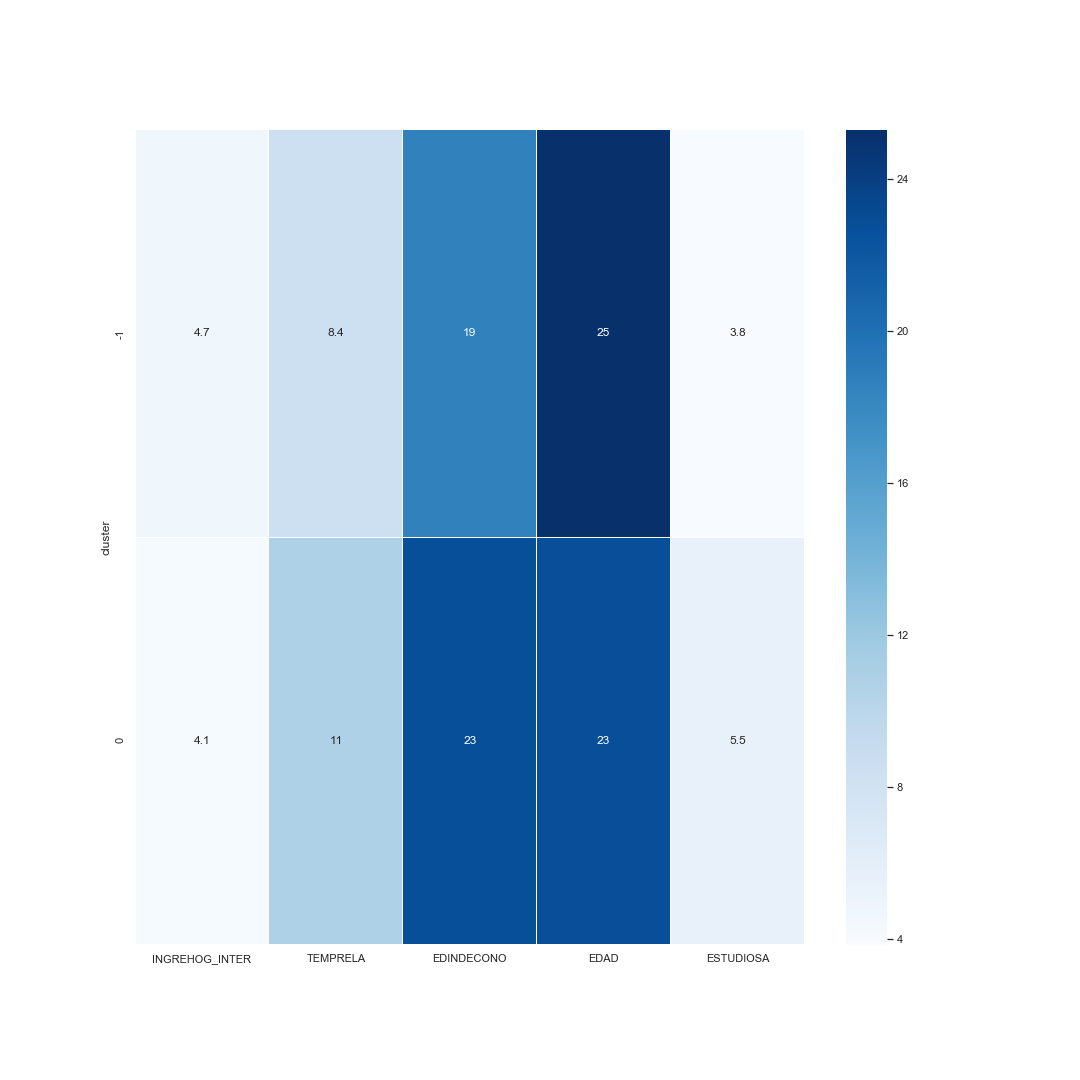
\includegraphics[width=0.55\textwidth]{../img/heatmap/Caso3-DBSCAN.png}}
		
	\end{figure}
	
	
	\begin{figure}[H]
		\centering
		\subfloat[MeanShift]{
			\label{f:MeanShift}
			\includegraphics[width=0.55\textwidth]{../img/heatmap/Caso3-MeanShift.png}}
		\subfloat[KMeans]{
			\label{f:KMeans}
			\includegraphics[width=0.55\textwidth]{../img/heatmap/Caso3-KMeans.png}}
		
		
	\end{figure}
	
	
	\begin{figure}[H]
		\centering
		\subfloat[MiniBatchKM]{
			\label{f:MiniBatchKM}
			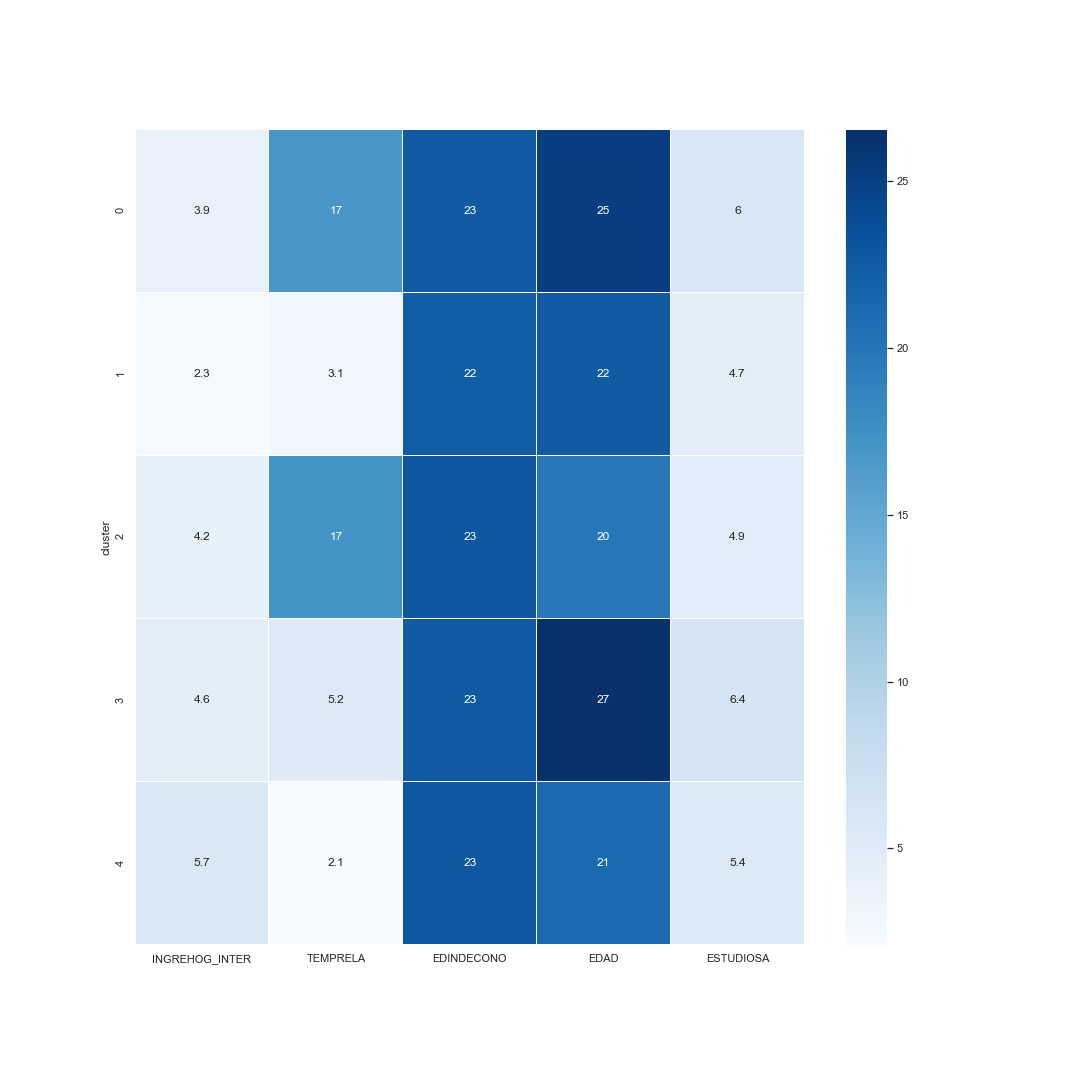
\includegraphics[width=0.75\textwidth]{../img/heatmap/Caso3-MiniBatchKM.png}}
		
	\end{figure}

	Observamos en primer lugar el algoritmo DBSCAN, en el que tenemos 2 clusters.
	En el cluster superior, hay más ingresos que en el inferior, lo que se ve reflejada en una independencia económicamente de sus padres anterior, con 19 años frente a los 23 años. \\
	
	Pasemos a estudiar otro algoritmo con mayor número de clusters, por ejemplo \texttt{KMeans}. Como se muestra en los clusters 0 , 2 y 4, una mayor cantidad de ingresos no se ve reflejado en una mayor estabilidad con la pareja. \\
	Por otro lado, todos los clusters comparten una edad de independencia económica de los padres similar (en torno a los 23 años), por tanto, lo datos no parecen tener mucha relación o mejor dicho, no podemos sacar conclusiones claras.
	
	
	\newpage
	\subsection{Dendogram}
	
	Mostramos ahora el dendograma resultante tras la ejecución:
	
	\begin{figure}[H]
		\centering
		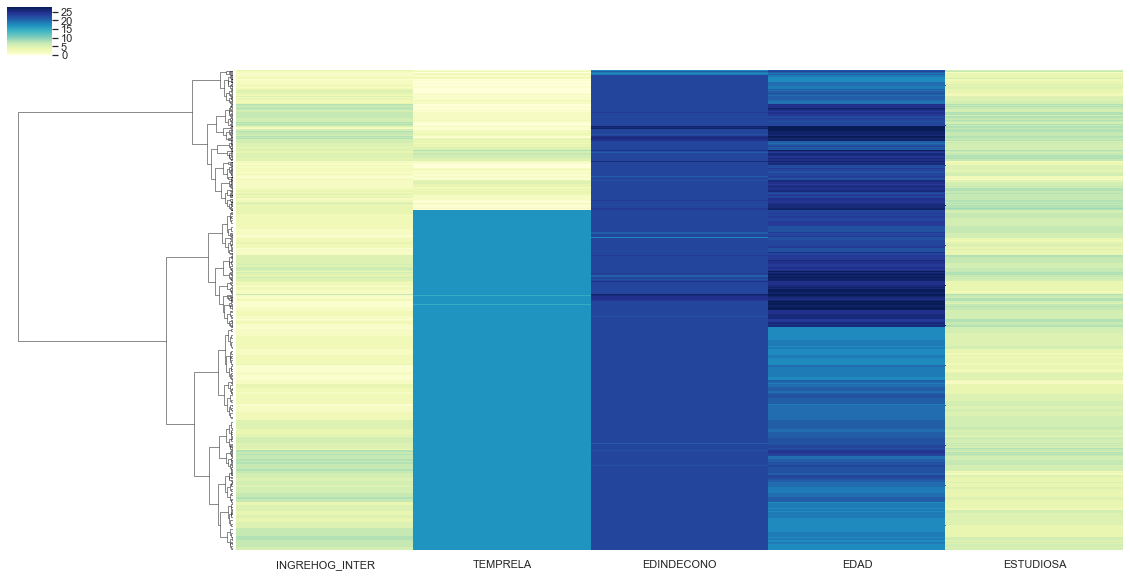
\includegraphics[scale=0.37]{../img/dendogram/Caso3-AgglomerativeClustering.png}
		
		\caption{Dendogram}
	\end{figure}
	
	
	
	\subsection{ScatterMatrix}
	
	Ahora bien, mostramos las Scatter Matrix de los diferentes algoritmos:
	
	\begin{figure}[H]
		\centering
		\subfloat[Agglo]{
			\label{f:Agglo}
			\includegraphics[width=0.55\textwidth]{../img/scatter/Caso3-AgglomerativeClustering.png}}
		\subfloat[DBSCAN]{
			\label{f:DBSCAN}
			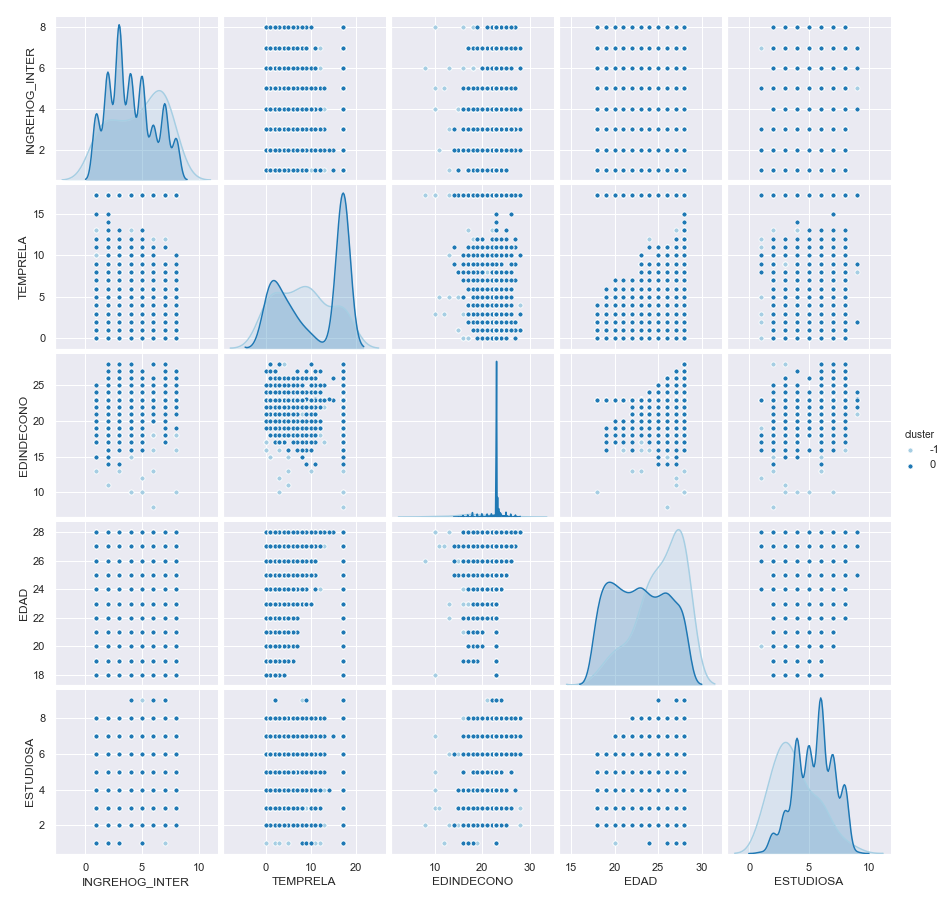
\includegraphics[width=0.55\textwidth]{../img/scatter/Caso3-DBSCAN.png}}
		
	\end{figure}
	
	
	\begin{figure}[H]
		\centering
		
		\subfloat[MiniBatchKM]{
			\label{f:MiniBatchKM}
			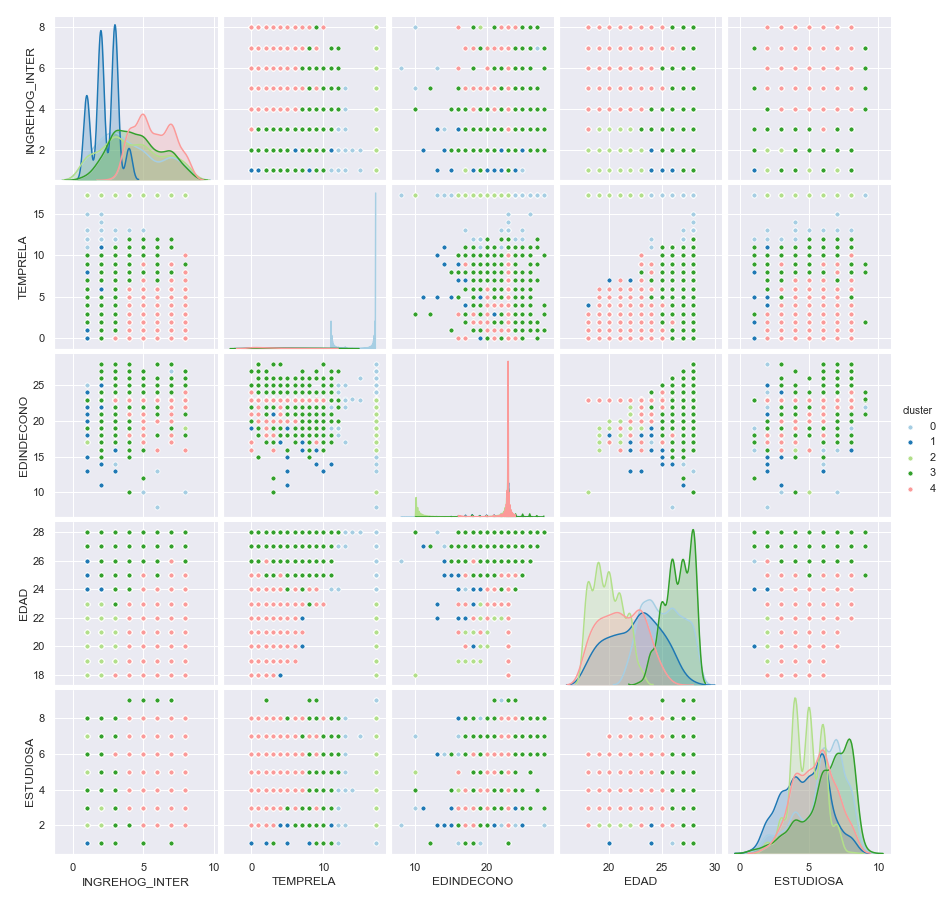
\includegraphics[width=0.55\textwidth]{../img/scatter/Caso3-MiniBatchKM.png}}
		\subfloat[KMeans]{
			\label{f:KMeans}
			\includegraphics[width=0.55\textwidth]{../img/scatter/Caso3-KMeans.png}}
		
		
	\end{figure}
	
	
	\begin{figure}[H]
		\centering
		\subfloat[MeanShift]{
			\label{f:MeanShift}
			\includegraphics[width=0.75\textwidth]{../img/scatter/Caso3-MeanShift.png}}
		
	\end{figure}

	\newpage

	\subsection{Kplot y BoxPlot}
	
	Por último, generamos un diagrama de densidad KPlot y un diagrama de caja BoxPlot, ambos comentados y explicados anteriormente:

	
	\begin{figure}[H]
		\centering
		\subfloat[KPlot - KMeans]{
			\label{f:KPlot - KMeans}
			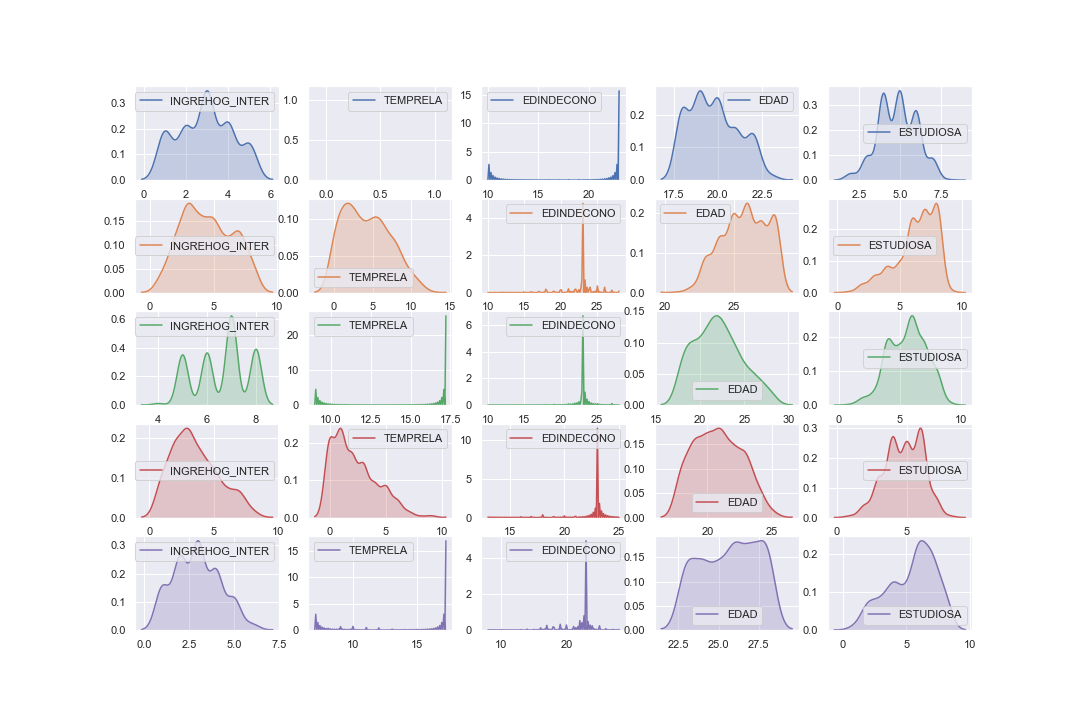
\includegraphics[width=1.16\textwidth]{../img/kplot/KMeans_3Kplot.png}}
		
	\end{figure}
	
	
	
	\begin{figure}[H]
		\centering
		\subfloat[BoxPlot - KMeans]{
			\label{f:BoxPlot - KMeans}
			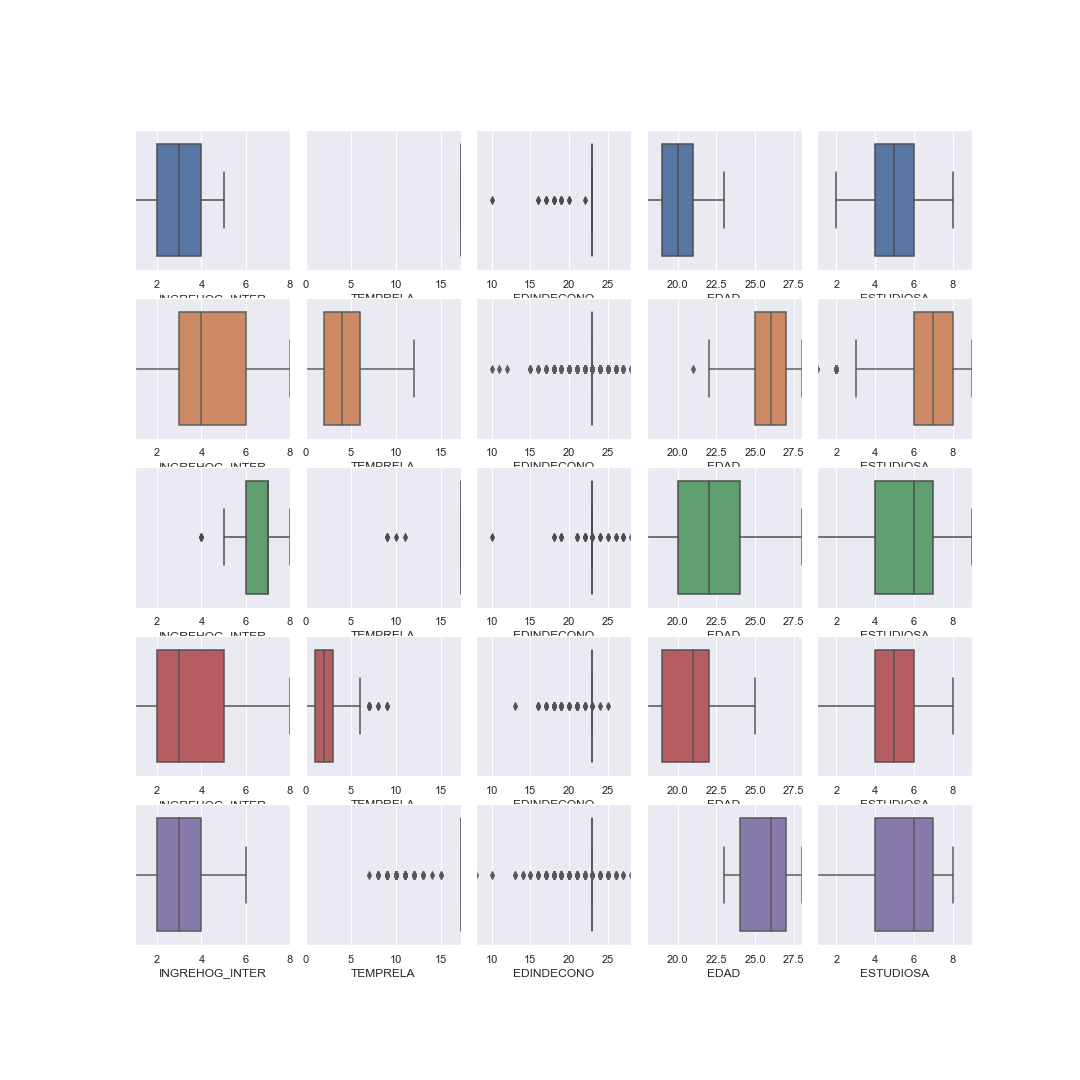
\includegraphics[width=1.05\textwidth]{../img/boxplot/KMeans_3boxplot.png}}
		
	\end{figure}
	
	
	
	\newpage
	
	\subsection{Interpretación de la segmentación}
	
	Por último, volcamos los datos en el fichero \texttt{caso\_3.txt}.
	
	Obtenemos del fichero los siguientes resultados:
	
	\begin{itemize}
		\item Tamaño de la muestra: 2927
		\item Se ha creado para cada algoritmo una tabla comparativa de los clusters y otra con el tamaño de cada cluster.
		\item Una tabla final con los resultados obtenidos:
	\end{itemize}
	
	
	\begin{table}[H]
		\centering
			\begin{tabular}{|l|l|l|l|l|}
				\hline
				\textbf{Algoritmo}               & \textbf{Número Clusters} & \textbf{SH} & \textbf{CH} & \textbf{Tiempo} \\ \hline
				\textbf{MeanShift}               & 2                        & 0.378570    & 1954.804484 & 1.702231        \\ \hline
				\textbf{KMeans}                  & 5                        & 0.285219    & 1342.770099 & 0.211653        \\ \hline
				\textbf{AgglomerativeClustering} & 5                        & 0.251886    & 1207.103682 & 0.959178        \\ \hline
				\textbf{MiniBatchKM}             & 5                        & 0.259901    & 1200.800644 & 0.144073        \\ \hline
				\textbf{DBSCAN}                  & 2                        & 0.106797    & 34.005134   & 0.289262        \\ \hline
			\end{tabular}%
		
	\end{table}

	Vemos que el mejor algoritmo es \texttt{MeanShift}. Es el que tarda un mayor tiempo en ejecutar pero el que saca mejores valores en las métricas \texttt{SH} y \texttt{CH}. El peor de todos es \texttt{DBSCAN}, con valores en las métricas muy bajos. 
	
	El resto de algoritmos se mantienen en la media pero mejoran el tiempo de ejecución de \texttt{Meanshift}. Cabe destacar que tanto el mejor como el peor algoritmo usan 2 clusters, por lo que el número de clusters entre algoritmos no se relacionan proporcionalmente. \\
	
	Mostramos ahora el tamaño de los clusters de \texttt{MeanShift}, el mejor algoritmo:
	
	\begin{table}[H]
			\centering
			\begin{tabular}{|l|l|}
				\hline
				\textbf{Cluster} & \textbf{Tamaño de cada cluster} \\ \hline
				\textbf{0:}      & 1518 (51.86\%)                   \\ \hline
				\textbf{1:}      & 1409 (48.14\%)                   \\ \hline
			\end{tabular}%
		
	\end{table}

	En ambos, la proporción de la muestra se mantiene prácticamente igual, en torno al 50\%
	
	
	
	\subsubsection{Modificaciones}
	
	Modificamos ahora los algoritmos \texttt{KMean} y \texttt{Agglomerative Clustering} y estudiamos el caso de estudio número 3.
	
	
	Para ambos estudiaremos los índices \texttt{Silhouette} y \texttt{Calinski Harabaz}, con 2 y 5 clusters, teniendo en cuenta que las proporciones se mantienen equilibradas.
	
	
	\newpage
	Obtenemos entonces:
	
	\begin{itemize}
		\item Tamaño de los clusters:
		
		\begin{table}[H]
		\centering
				\begin{tabular}{|l|l|l|l|l|}
					\cline{1-2} \cline{4-5}
					\textbf{Agglo5} & \textbf{Tamaño de cluster} & \multirow{6}{*}{} & \textbf{Kmean5} & \textbf{Tamaño de cluster} \\ \cline{1-2} \cline{4-5} 
					0:              & 965 (32.97\%)              &                   & 1:              & 747 (25.52\%)              \\ \cline{1-2} \cline{4-5} 
					3:              & 636 (21.73\%)              &                   & 0:              & 600 (20.50\%)              \\ \cline{1-2} \cline{4-5} 
					1:              & 528 (18.04\%)              &                   & 3:              & 581 (19.85\%)              \\ \cline{1-2} \cline{4-5} 
					2:              & 460 (15.72\%)              &                   & 4:              & 513 (17.53\%)              \\ \cline{1-2} \cline{4-5} 
					4:              & 338 (11.55\%)              &                   & 2:              & 486 (16.60\%)              \\ \cline{1-2} \cline{4-5} 
				\end{tabular}%
			
		\end{table}
		
		
		
		\begin{table}[H]
		\centering
				\begin{tabular}{|l|l|l|l|l|}
					\cline{1-2} \cline{4-5}
					\textbf{Agglo2} & \textbf{Tamaño de cluster} &  & \textbf{Kmean2} & \textbf{Tamaño de cluster} \\ \cline{1-2} \cline{4-5} 
					1:              & 1502 (51.32\%)             &  & 1:              & 1514 (51.73\%)             \\ \cline{1-2} \cline{4-5} 
					0:              & 1425 (48.68\%)             &  & 0:              & 1413 (48.27\%)             \\ \cline{1-2} \cline{4-5} 
				\end{tabular}%
			
		\end{table}
	
		En general, podemos afirmar que las proporciones se mantienen más o menos iguales.
		
		
		\item Resultados obtenidos:
		
		\begin{table}[H]
		\centering
				\begin{tabular}{|l|l|l|l|l|}
					\hline
					\textbf{Algoritmo} & \textbf{Número Clusters} & \textbf{SH} & \textbf{CH} & \textbf{Tiempo} \\ \hline
					Agglo\_5           & 5                        & 0.251886    & 1207.103682 & 0.912252        \\ \hline
					Agglo\_2           & 2                        & 0.378041    & 1950.009582 & 0.914670        \\ \hline
					KMeans\_5          & 5                        & 0.285219    & 1342.770099 & 0.197634        \\ \hline
					KMeans\_2          & 2                        & 0.378626    & 1955.356642 & 0.062568        \\ \hline
				\end{tabular}%
			
		\end{table}
	
		Vemos que en los dos algoritmos, para \textit{n\_clusters = 2} se obtienen mejores resultados que para usando \textit{n\_clusters = 5}. Además, el tiempo de ejecución disminuye. 
		
		
	\end{itemize}

\newpage 
	\section{Contenido adicional}
	
	En esta sección explicaremos algunos conceptos importantes que se usan en la práctica y requieren algún comentario
	
	
	\subsection{Normalización}
	
	Debido a los diferentes rangos de las variables y paso previo a la ejecución de los algoritmos, los datos han sido normalizados:
	
	\begin{lstlisting}[frame=single]
def norm_to_zero_one(df):
	return (df - df.min()) * 1.0 / (df.max() - df.min())
	\end{lstlisting}
	
	
	
	
	
	
	\subsection{Estudio de valores perdidos}
	La base de datos proporcionada para la realización de la práctica, posee algunos valores perdidos que hemos tenido que rellenar.
	
	Como primera opción, se pueden reemplazar los valores desconocidos por un número:
	\begin{lstlisting}[frame=single]
datos = datos.replace(np.NaN,0)
	\end{lstlisting}
	
	Por otro lado, y como mejor opción elegida, imputamos con la media:
	
	\begin{lstlisting}[frame=single]
for col in data:
	data[col].fillna(data[col].mean(), inplace=True)
	
	\end{lstlisting}
	
	Al imputar con la media, nos quedamos con un valor que seguramente se acerque más al valor real, que es mucho mejor que directamente poner un 0.
	
	
	
	
	
	
	\newpage
	
	\section{Bibliografía}
	
	
	
	
	
	

	
	
	
	% -----------------------------------------------
	% Bibliografía.
	% -----------------------------------------------
	\begin{thebibliography}{9}
		
		
	\bibitem{Página web de la asignatura - http://sci2s.ugr.es/graduateCourses/in}
	\href{}{Página web de la asignatura - http://sci2s.ugr.es/graduateCourses/in}
		
	\bibitem{http://scikit-learn.org/stable/modules/clustering.html}
	\href{}{http://scikit-learn.org/stable/modules/clustering.html}
	
		
		
			
	
		
		
		
		\end{thebibliography}
	
	
	
	

		
	\end{document}